% =============================================================================
%  Projet de Fin d'Études (PFE)
%  Distributed Vehicle Detection using Stereo Cameras and V2V Communication
%  Master document — compiles all chapters
%
%  Build:  pdflatex main  ->  bibtex main  ->  pdflatex main  ->  pdflatex main
%  Engine: pdfLaTeX (all figures are native TikZ; no Unicode art)
% =============================================================================
\documentclass[12pt,a4paper,oneside]{report}

% ---- Encoding & fonts -------------------------------------------------------
\usepackage[utf8]{inputenc}
\usepackage[T1]{fontenc}
\usepackage{lmodern}
\usepackage[english]{babel}
\usepackage{microtype}

% ---- Page geometry & spacing ------------------------------------------------
\usepackage[a4paper,inner=3.0cm,outer=2.5cm,top=2.5cm,bottom=2.5cm]{geometry}
\usepackage{setspace}
\onehalfspacing
\usepackage{emptypage}

% ---- Mathematics ------------------------------------------------------------
\usepackage{amsmath}
\usepackage{amssymb}
\usepackage{amsfonts}
\usepackage{bm}

% ---- Tables -----------------------------------------------------------------
\usepackage{booktabs}
\usepackage{tabularx}
\usepackage{array}
\usepackage{multirow}
\usepackage{makecell}
\renewcommand\theadfont{\bfseries}
\renewcommand\theadalign{cc}
\newcolumntype{L}{>{\raggedright\arraybackslash}X}

% ---- Figures & graphics -----------------------------------------------------
\usepackage{graphicx}
\usepackage{float}
\usepackage[font=small,labelfont=bf,width=.92\textwidth]{caption}
\usepackage{tikz}
\usetikzlibrary{arrows.meta,positioning,calc,shapes.geometric,fit,backgrounds,decorations.pathreplacing}

% ---- Lists & misc -----------------------------------------------------------
\usepackage{enumitem}
\usepackage{xcolor}
\usepackage{tcolorbox}

% ---- Headers / footers ------------------------------------------------------
\usepackage{fancyhdr}
\pagestyle{fancy}
\fancyhf{}
\renewcommand{\headrulewidth}{0.4pt}
\fancyhead[L]{\nouppercase{\leftmark}}
\fancyhead[R]{\thepage}
\fancypagestyle{plain}{\fancyhf{}\fancyfoot[C]{\thepage}\renewcommand{\headrulewidth}{0pt}}

% ---- Bibliography (numeric IEEE-style, matches the SOTA draft) ---------------
\usepackage[numbers,sort&compress]{natbib}
\bibliographystyle{ieeetr}

% ---- Hyperlinks (load late) -------------------------------------------------
\usepackage[hidelinks,breaklinks=true]{hyperref}
\hypersetup{
  colorlinks=true,
  linkcolor=black,
  citecolor=black,
  urlcolor=blue!55!black,
  pdftitle={Distributed Vehicle Detection using Stereo Cameras and V2V Communication},
  pdfauthor={Ijja Baq}
}
\usepackage[capitalise,noabbrev]{cleveref}

% ---- Custom TikZ styles shared across chapters ------------------------------
\tikzset{
  stagebox/.style   ={draw,rounded corners,align=center,font=\small,
                       minimum width=2.9cm,minimum height=1.0cm,fill=blue!6},
  databox/.style    ={draw,align=center,font=\footnotesize,
                       minimum width=2.6cm,minimum height=0.8cm,fill=gray!8},
  fusebox/.style    ={draw,thick,rounded corners,align=center,font=\small,
                       minimum width=3.4cm,minimum height=1.2cm,fill=orange!12},
  vbox/.style       ={draw,rounded corners,align=center,font=\footnotesize,
                       minimum width=3.6cm,minimum height=1.0cm},
  flow/.style       ={-{Latex[length=2.2mm]},thick},
  corr/.style       ={dashed,{Latex[length=1.6mm]}-{Latex[length=1.6mm]},gray!70!black},
}

% =============================================================================
\begin{document}

% ----------------------------- Front matter ----------------------------------
% ----------------------------- Title page ------------------------------------
\begin{titlepage}
\centering
\thispagestyle{empty}

{\scshape\large Université Ibn Zohr\par}
{\scshape Faculté des Sciences\par}
\vspace{0.4cm}
{\large Projet de Fin d'Études (PFE)\par}
\vspace{0.2cm}
\rule{\textwidth}{0.4pt}

\vfill

{\Huge\bfseries Distributed Vehicle Detection using\\[0.35em]
Stereo Cameras and V2V Communication\par}
\vspace{0.8cm}
{\large\itshape A Cooperative Late-Fusion Perception Pipeline\\
Built on Passive Stereo Sensing\par}

\vfill

\begin{minipage}{0.45\textwidth}
\begin{flushleft}\large
\textbf{Author:}\\
Ijja \textsc{Baq}
\end{flushleft}
\end{minipage}
\hfill
\begin{minipage}{0.45\textwidth}
\begin{flushright}\large
\textbf{Supervisor:}\\
Prof. \textsc{[Supervisor Name]}
\end{flushright}
\end{minipage}

\vfill

\rule{\textwidth}{0.4pt}
{\large A thesis submitted in partial fulfilment of the requirements\\
for the degree of Engineering / Master\par}
\vspace{0.6cm}
{\large \today\par}

\end{titlepage}


\pagenumbering{roman}

\cleardoublepage
\phantomsection
\addcontentsline{toc}{chapter}{Abstract}
% ------------------------------- Abstract ------------------------------------
\chapter*{Abstract}
\markboth{Abstract}{Abstract}

Cooperative perception lets connected vehicles extend their sensing horizon
beyond the line of sight by exchanging spatial information over
Vehicle-to-Vehicle (V2V) links. Existing benchmarks, however, almost universally
assume LiDAR as the sensing modality, leaving the feasibility of cooperation
built on low-cost \emph{passive stereo} cameras uncharacterised. This thesis
investigates whether a cooperative perception system relying exclusively on
stereo cameras can yield a measurable and characterisable improvement in
three-dimensional localisation over single-agent stereo perception, and what the
operating limits of such an approach are.

A four-stage pipeline is proposed and validated under a V-model development
process: dense stereo depth estimation, 2D object detection, lifting of
detections to 3D position, and a decentralised object-level (late) fusion layer
that registers and merges the independent observations of two cooperating
agents. Guided by the range-dependent, quadratically growing error of stereo
triangulation, the single-vehicle chain deliberately outputs 3D \emph{position}
rather than full 3D bounding boxes. A dual-dataset strategy exercises the
single-vehicle chain on real driving stereo imagery (KITTI) and the cooperative
layer on simultaneous, occlusion-truthful multi-agent recordings from the CARLA
simulator.

Empirical characterisation shows that the headline benefit of stereo
cooperation is \emph{coverage} rather than localisation: late fusion recovers
objects hidden in each agent's blind spots and raises recall substantially for
both agents symmetrically, while localisation error remains essentially flat
because the two viewpoints share a narrow viewing-angle separation that
precludes effective triangulation. The work thus establishes a baseline for
late fusion operating strictly on stereo-sourced inputs and maps the conditions
under which cooperative gains hold.

\vspace{0.6cm}
\noindent\textbf{Keywords:} cooperative perception, V2V communication, stereo
vision, depth estimation, 3D object localisation, late fusion, autonomous
driving, KITTI, CARLA.


\cleardoublepage
\tableofcontents
\listoffigures
\listoftables

% ------------------------------ Main matter ----------------------------------
\cleardoublepage
\pagenumbering{arabic}

\chapter{Introduction}
\label{ch:introduction}

\section{Context and Motivation}

The rapid evolution of Advanced Driver Assistance Systems (ADAS) and autonomous
driving architectures has progressively shifted the modern automotive industry
toward sensor-driven autonomy. Production vehicles are increasingly equipped with
ADAS functionalities such as adaptive cruise control, autonomous emergency
braking, and lane-keeping assistance, which actively mitigate human error and
improve traffic safety~\cite{yurtsever2020}. These systems depend entirely on
robust, real-time perception pipelines capable of constructing an accurate
three-dimensional representation of the surrounding environment. Perception is
not one module among many in an autonomous system: it is the entry point through
which all subsequent reasoning, planning, and control decisions flow, and
failures at this stage propagate irreversibly downstream.

Despite significant advances in single-agent perception, the standalone paradigm
faces a physical constraint that no algorithmic improvement can resolve: a single
vehicle cannot perceive beyond its line of sight. Occlusions behind large
commercial vehicles, blind intersections, and vehicles emerging from concealed
driveways represent everyday driving scenarios that leave autonomous systems
unaware of hazards until they enter the immediate sensor field of the
ego-vehicle. Cooperative perception addresses this at its root: by exchanging
spatial data over V2V communication networks, connected vehicles collectively
extend their sensing horizon beyond what any individual agent could achieve,
resolving blind spots through complementary viewpoints rather than better onboard
processing.

Deploying such a system at scale, however, raises an immediate practical question
of sensing modality. High-definition Light
Detection and Ranging (LiDAR) scanners have dominated the academic
literature due to their direct 3D measurements, but their cost, power
consumption, and mechanical complexity remain significant barriers to mass-market
deployment. Passive stereo camera arrays offer a compelling alternative: metric
depth recovery through geometric triangulation, without active illumination.
Their hardware cost and form factor are compatible with large-scale fleet
integration, making them a practical sensing backbone for cooperative systems.

It is this combination --- cooperative perception built on passive stereo
sensing --- that this project investigates.

\section{Problem Statement}

Deploying cooperative perception on passive stereo cameras raises a fundamental
feasibility concern. Stereo depth estimation recovers metric distance through
geometric triangulation, and its localisation error does not scale linearly with
range but quadratically. An object detected at 50 metres carries substantially
higher positional uncertainty than the same object detected at 15
metres~\cite{huang2025}. This range-dependent degradation means that the quality
of a stereo-sourced 3D detection is not a fixed property of the detector but a
function of where the target is relative to the sensing vehicle.

In a cooperative setting, this property becomes a structural problem. When two
stereo-equipped vehicles observe the same target from different distances, the
detections they produce carry fundamentally different uncertainty profiles.
Merging them into a unified environmental model requires reconciling estimates
whose reliability varies not just between agents but across the operational range
of each agent individually. Whether the geometric complementarity of two
viewpoints is sufficient to produce a net improvement in localisation accuracy,
and under what distance conditions that improvement holds or collapses, is not
established in the literature. Existing cooperative perception benchmarks and
evaluation frameworks assume LiDAR as the primary sensing modality, leaving the
stereo operating regime without a direct empirical
reference~\cite{xu2023v2v4real}.

The central question this work addresses is whether a cooperative perception
system built exclusively on passive stereo cameras can produce a measurable and
characterisable improvement in 3D localisation over single-agent stereo
perception, and what the operating limits of such an approach are.

\section{Research Objectives}

To evaluate how object-level late fusion handles range-dependent stereo noise,
this research defines three primary engineering and analytical objectives:

\begin{enumerate}[label=\textbf{O\arabic*.},leftmargin=*,itemsep=4pt]
  \item \textbf{Development of a Single-Agent 3D Spatial Localisation Baseline.}
  Implement a stereo vision pipeline that pairs 2D object detection with passive
  stereo depth estimation to project image-plane detections into a
  three-dimensional metric space. The objective is to establish the per-agent
  detection quality and localisation accuracy that feed into the cooperative
  layer.

  \item \textbf{Design of a Decentralised Object-Level Fusion Layer.} Construct a
  modular Vehicle-to-Vehicle (V2V) late fusion architecture that operates
  independently of agent software backbones. This module ingests 3D position
  estimates from multiple collaborating nodes, resolves the geometric
  transformations required to align independent coordinate frames, and merges
  redundant detections into a unified scene representation.

  \item \textbf{Empirical Characterisation of Cooperative Localisation
  Dynamics.} Conduct systematic experiments within real-world benchmark
  sequences and simulated multi-vehicle environments to map the performance
  profile of the cooperative stack. The focus is to quantify how spatial
  localisation error, precision, and recall evolve with increasing target
  distance, and to analyse how late fusion logic behaves when aggregating depth
  estimates from classical and learned stereo engines across agents.
\end{enumerate}

\section{Thesis Structure}

The remainder of this document is organised as follows to address these
objectives:

\begin{itemize}[leftmargin=*,itemsep=3pt]
  \item \textbf{Chapter~\ref{ch:sota}: Literature Review and State-of-the-Art}
  surveys existing work in stereo depth estimation, 3D spatial localisation, and
  collaborative perception to establish the boundaries of current research.
  \item \textbf{Chapter~\ref{ch:methodology}: Methodology and Proposed
  Framework} details the end-to-end engineering architecture of the pipeline and
  the V-model development process adopted to structure the design,
  implementation, and validation phases of the system.
  \item \textbf{Chapter~\ref{ch:experimental}: Experimental Setup and Simulation
  Environment} outlines the dataset configurations, simulated CARLA scenarios, and
  specific evaluation metrics used to test the system.
  \item \textbf{Chapter 5: Results and Discussion} presents the empirical data,
  performance plots, and the precision--recall trade-offs discovered during
  testing.
  \item \textbf{Chapter 6: Conclusion and Future Work} summarises the core
  findings, addresses current system limitations, and outlines future research
  pathways.
\end{itemize}

\chapter{Literature Review and State-of-the-Art}
\label{ch:sota}

Environmental perception in autonomous driving has evolved substantially since
the early rule-based systems, progressing from monocular detection pipelines on
individual vehicles toward fully learned, multi-agent systems capable of
reasoning about shared perceptual information in real time. Modern cooperative
perception sits at the intersection of three distinct research fields that have
individually achieved significant maturity: stereo-based 3D perception, deep
learning for object detection, and collaborative perception networks. This
chapter surveys the current state of the art across each of these three domains,
tracing the trajectory of each field and identifying where the boundaries of
current methods lie.

\section{Stereo-Based 3D Perception}
\label{sec:stereo3d}

Autonomous driving platforms require a real-time, metric three-dimensional
representation of their surroundings before any higher-level task such as object
tracking, trajectory prediction, or path planning can proceed reliably. How that
representation is obtained from onboard sensors is a non-trivial design choice,
and one that has shifted considerably as the field has matured. This section
examines the principal sensing paradigms in autonomous perception, then traces
the algorithmic evolution of stereo depth estimation methods.

\subsection{Sensor Modalities}

To capture the spatial layout of an environment, modern autonomous perception
systems primarily utilise one of three core sensor configurations: active LiDAR arrays, passive monocular cameras, or passive
stereo cameras. Each modality presents a fundamentally distinct engineering
compromise across financial cost, hardware reliability, semantic density, and
geometric depth accuracy~\cite{valverde2025}.

Active sensing via LiDAR has long served as the benchmark for metric 3D
perception. By emitting localised infrared laser pulses and calculating the
direct Time-of-Flight (ToF) of their reflections, LiDAR sensors generate sparse
but highly accurate point clouds that are largely invariant to ambient lighting
conditions or shadows. This direct coordinate measurement eliminates downstream
geometric ambiguity, providing high metric precision at ranges exceeding one
hundred metres. Despite these geometric advantages, active LiDAR sensing suffers
from severe operational constraints: high-resolution automotive units remain
prohibitively expensive for mass-market deployment, carry significant power
consumption, rely on mechanical or solid-state components vulnerable to physical
wear, and produce point clouds inherently devoid of semantic texture, rendering
them incapable of capturing colour, reading signage, or interpreting traffic
state.

Conversely, monocular camera systems offer the most affordable and
computationally streamlined alternative for automotive perception. Single cameras
provide dense, high-resolution RGB images that contain rich semantic textures,
allowing deep neural networks to classify objects, detect lane boundaries, and
interpret complex scene contexts. However, extracting 3D metric coordinates from
a single 2D image plane is a mathematically ill-posed inverse problem. Because
the projection from a 3D world space to a 2D pixel grid discards the depth
dimension entirely, monocular systems suffer from fundamental scale
ambiguity~\cite{huang2025monocular}. To estimate distance, monocular deep
learning models must rely heavily on statistical priors and contextual cues
learned during training, such as assuming a vehicle's standard height or
ground-plane consistency. Consequently, when confronted with out-of-distribution
obstacles, unusual vehicle profiles, or severe ego-vehicle pitch, these models
degrade substantially, with published depth errors typically falling in the
15--30\% range and accuracy degrading further beyond 50 metres as perspective
cues become insufficient to resolve absolute scale~\cite{huang2025}.

Stereo vision recovers absolute metric depth through passive geometric
triangulation across two synchronised, horizontally offset cameras separated by a
fixed known baseline, requiring no learned priors about object appearance or
scale. This geometry preserves the dense semantic richness and low hardware cost
of camera-based sensing while establishing a physically grounded foundation for
depth recovery. Unlike learned monocular approaches, stereo triangulation is
distribution-agnostic: it applies equally to any rigid object in the scene
regardless of whether that object class appeared in the depth model's training
data, making it a practical and scalable baseline for single-agent 3D perception
in cost-constrained deployments~\cite{huang2025}.

\subsection{Stereo Depth Estimation}
\label{sec:stereodepth}

Extracting reliable depth from a stereo pair requires solving a precise geometric
problem that has driven decades of algorithmic development. The foundational
objective of a computational stereo engine is to solve the correspondence
problem: identifying the exact spatial location of a point in a secondary camera
frame that matches a given pixel in the primary camera frame. By assuming a
rectified camera arrangement where the optical axes are parallel, the search
space for a matching pixel can be mathematically constrained from a
two-dimensional grid to a one-dimensional horizontal epipolar line. The
horizontal pixel displacement between these matched points represents the
disparity, which inversely determines the absolute metric depth of the scene
relative to the camera's baseline and focal length.

Historically, the computer vision literature divided dense disparity estimation
into local and global optimisation paradigms~\cite{scharstein2002}. Local
methods, such as Block Matching (BM), compute correspondence costs over isolated
support windows using pixel-level intensity metrics. While computationally
efficient, local matching degrades significantly in textureless regions or under
uniform illumination. Global matching paradigms address these spatial ambiguities
by introducing mathematical energy minimisation functions. Algorithms like
Semi-Global Matching (SGM)~\cite{hirschmuller2008} approximate global 2D
optimisation by aggregating dynamic programming paths across multiple 1D
orientations through the image grid. SGM balances per-pixel matching accuracy
with contextual smoothness constraints, making it a practical baseline for
real-time stereo matching in robotics and automotive applications. However, it
still exhibits severe optimisation failures when confronted with reflective
materials, fine structural boundaries, or repeated patterns.

The integration of deep learning drastically shifted the stereo landscape by
replacing hand-crafted cost functions with data-driven representations.
Influential deep architectures such as PSMNet~\cite{chang2018} introduced the
concept of the 3D visual cost volume. Instead of matching raw pixel intensities,
these networks employ Siamese Convolutional Neural Networks (CNNs) to extract
dense feature descriptors from both views, which are concatenated across a range
of predefined candidate disparities to construct a high-dimensional cost volume.
Volumetric 3D convolutions are then applied to aggregate spatial and disparity
context over the volume to regress a smooth disparity map.

To refine this volumetric approach, the field transitioned toward iterative
recurrent architectures, an approach exemplified by RAFT-Stereo~\cite{lipson2021}.
RAFT-Stereo extracts multi-scale feature maps, constructs a multi-scale 4D
correlation cost volume, and utilises a Gated Recurrent Unit (GRU) block to
iteratively look up and update the disparity field. While RAFT-Stereo achieved
unprecedented accuracy on fine structures across major benchmarks, maintaining
and fetching data from multi-scale 4D cost volumes still imposes significant
memory bottlenecks on embedded automotive hardware.

To completely bypass the computational overhead imposed by volumetric
representations, contemporary research has shifted toward cost-volume-free,
recurrent warping architectures, an approach exemplified by
WAFT-Stereo~\cite{wang2026}. Rather than building or maintaining a static,
memory-heavy cost structure, WAFT-Stereo frames stereo matching as a continuous
field transformation, iteratively warping feature maps from one view directly
onto the other and utilising localised field transforms to resolve geometric
misalignments progressively. By relying strictly on high-resolution warping
mechanisms rather than dense volumetric convolutions or correlation lookups, this
framework holds a top-ranking position on ETH3D, Middlebury, and KITTI across all
metrics, while running 1.8 to 6.7 times faster than competitive
methods~\cite{wang2026}, providing a highly scalable depth engine for downstream
detection tasks.

\Cref{tab:stereo} provides a comparative summary of this algorithmic evolution
across four representative methodologies, contrasting their core paradigms, error
metrics on the KITTI 2015 benchmark, operational latencies, and deployment
hardware configurations.

\begin{table}[ht]
\centering
\caption{Representative stereo depth estimation methods on the KITTI 2015 benchmark.}
\label{tab:stereo}
\renewcommand{\arraystretch}{1.6}
\small
\resizebox{\textwidth}{!}{%
\begin{tabular}{l l c c l}
\toprule
\thead{Method} & \thead{Paradigm} &
\thead{KITTI 2015 \\ D1-all} &
\thead{Latency} & \thead{Hardware} \\
\midrule
SGBM \cite{hirschmuller2008}
  & Classical path aggregation
  & $\sim$8--12\% & $<$25\,ms & Multi-core CPU \\[4pt]
PSMNet \cite{chang2018}
  & CNN + 3D cost volume
  & 2.32\% & $\sim$410\,ms & NVIDIA GTX 1080Ti \\[4pt]
RAFT-Stereo \cite{lipson2021}
  & Recurrent + 4D correlation volume
  & 2.42\% & $\sim$380\,ms & NVIDIA RTX 3090 \\[4pt]
WAFT-Stereo \cite{wang2026}
  & Recurrent + feature warping (no cost volume)
  & 1.28\% & $\sim$100\,ms & NVIDIA L40 \\
\bottomrule
\end{tabular}}
\end{table}





\section{Single-Vehicle 3D Object Detection}
\label{sec:single3d}

Once a dense depth map is generated from the ego-vehicle's stereo vision engine,
the perception pipeline must use this depth information to localise and classify
surrounding vehicles. Single-vehicle 3D object detection focuses on predicting a
bounding box defined by a seven-degree-of-freedom state vector: a 3D centre
coordinate $(x, y, z)$, physical dimensions (height, width, length), and an
orientation angle (yaw). Within the autonomous vehicle literature, deep
architectures handle this localisation task through two fundamentally distinct
structural strategies. The first is a multi-stage lifting paradigm, which relies
on an explicit 2D image-plane detector to isolate objects before projecting them
into 3D coordinates using calculated depth data. The second is an end-to-end
paradigm encompassing volumetric and transformer-based architectures, which
bypasses intermediate 2D detections entirely, directly mapping raw stereo inputs
to 3D spatial parameters. This section first evaluates the core 2D detection
architectures that serve as the front-end for lifting workflows, before examining
both multi-stage pseudo-LiDAR approaches and end-to-end direct regression
systems.

\subsection{2D Object Detection as a Front-End for 3D Lifting}

In multi-stage perception frameworks, a 2D image-plane detector serves as a
structural prerequisite: it must first isolate objects within the RGB image
plane, whose boundaries are then used to crop depth maps and define the spatial
frustum passed to the 3D lifting stage. Because any localisation error at this
stage directly bounds the accuracy of the entire pipeline, the choice of 2D
backbone carries significant architectural weight. The literature primarily
offers three configurations for image-plane localisation: classical two-stage
proposal networks, modern single-shot convolutional networks, and real-time
end-to-end vision transformers.

The canonical two-stage detection baseline is Faster R-CNN~\cite{ren2015}. This
architecture established the foundational paradigm of separating localisation into
a sequential processing pipeline. The first stage employs a dedicated Region
Proposal Network (RPN) to scan dense feature maps and generate coarse bounding
box candidates. The second stage then utilises region-of-interest (RoI) pooling
layers to extract these features, passing them to downstream heads for final
categorical classification and bounding box regression. While Faster R-CNN
consistently achieved superior localisation precision and robust handling of
multi-scale objects compared to single-stage methods of the same period, its
multi-stage design introduces computational bottlenecks on embedded hardware,
making real-time deployment on automotive hardware challenging.

To address these latency constraints, the field shifted toward one-stage,
single-shot detectors, exemplified by the YOLO family (You Only Look
Once)~\cite{redmon2016}. One-stage architectures eliminate the region proposal
step entirely, framing object localisation as a direct, end-to-end regression
problem over a dense spatial grid. While early iterations relied on rigid,
hand-crafted anchor boxes that struggled with objects of varying scales and
aspect ratios, the family has evolved continuously, progressively adopting
anchor-free regression heads and increasingly expressive backbone designs. The
most recent iteration, YOLOv12, builds on this trajectory by introducing a
lightweight area attention module and a Residual Efficient Layer Aggregation
Network (R-ELAN), achieving incremental mAP gains over its predecessor while
matching its inference speed on standard GPU hardware~\cite{tian2025}, continuing
to narrow the historical trade-off between inference speed and detection accuracy.

Beyond convolutional architectures, contemporary multi-stage frameworks have
increasingly adopted Vision Transformers (ViTs), specifically the DETR (DEtection
TRansformer) lineage, as their localisation engine~\cite{carion2020}. While
convolutional models rely on localised receptive fields and hand-crafted
post-processing heuristics like Non-Maximum Suppression (NMS) to clear out
redundant, overlapping boxes, DETR models frame 2D localisation as a direct
set-prediction problem. Utilising multi-head self-attention mechanisms, these
networks capture global contextual dependencies and long-range cross-object
interactions across the entire image plane, matching learned object queries to
ground-truth boxes via bipartite matching. With modern adaptations like
RT-DETR~\cite{lv2024} drastically optimising the computational latency of these
attention maps, transformer-based frameworks produce exceptionally clean,
precisely bounded region crops without spatial suppression artefacts, a property
that directly improves the quality of the depth frustum passed to the 3D lifting
stage.

\Cref{tab:detectors} compares the three architectural families across detection
accuracy, inference latency, and primary deployment context. Latency values for
YOLOv12 and RT-DETR are measured using TensorRT FP16 (TRT FP16) optimisation on
an NVIDIA T4 GPU; Faster R-CNN latency is measured in standard PyTorch on a server
GPU.

\begin{table}[ht]
\centering
\caption{Comparison of major 2D object detection models on the COCO benchmark.}
\label{tab:detectors}
\renewcommand{\arraystretch}{1.6}
\small
\resizebox{\textwidth}{!}{%
\begin{tabular}{l l c c l}
\toprule
\thead{Model} & \thead{Family} &
\thead{COCO \\ mAP@0.5:0.95} &
\thead{Latency} & \thead{Design Priority} \\
\midrule
Faster R-CNN \cite{ren2015}
  & Two-stage proposal
  & $\sim$37\% & 100--200\,ms & Precision-first, latency-tolerant \\[4pt]
YOLOv12 \cite{tian2025}
  & One-stage anchor-free + attention
  & $\sim$51.8\% & $\sim$2.5\,ms TRT FP16 & Speed-first, edge deployment \\[4pt]
RT-DETR \cite{lv2024}
  & Transformer set prediction
  & $\sim$53.0\% & $\sim$9.3\,ms TRT FP16 & Transformer precision at real-time speed \\
\bottomrule
\end{tabular}}
\end{table}

\subsection{Stereo-Based 3D Object Detection}

While image-plane analysis extracts rich two-dimensional semantic maps,
autonomous vehicles require structural reasoning in native three-dimensional
coordinate frames. Resolving the extra spatial dimension from stereo camera
setups has produced two structurally distinct paradigms in the literature, driven
by a fundamental tension between geometric interpretability and end-to-end
computational efficiency.

\paragraph{a. Two-Stage Lifting and Pseudo-LiDAR Approaches.}
The two-stage lifting paradigm connects image-plane processing to 3D geometric
interpretation by decoupling the pipeline into explicit depth generation and
point-cloud detection components. This approach was popularised through the
Pseudo-LiDAR framework~\cite{wang2019pseudolidar}, which applies back-projection
to estimated disparity maps. Utilising camera calibration matrices, the network
converts every pixel with a known depth value directly into a concrete 3D point
cloud within the physical world coordinate frame. Once this coordinate
transformation occurs, the generated Pseudo-LiDAR point cloud mimics the
structural format of LiDAR point clouds. Consequently, these architectures can
directly deploy existing 3D point-cloud detection models, such as
PointRCNN~\cite{shi2019}, to group spatial points and regress 3D bounding boxes.
Subsequent iterations like Pseudo-LiDAR++ refined this by using sparse physical
measurements to correct depth errors, which naturally scale quadratically with
actual physical distance~\cite{you2020}. While this explicit separation makes the
overall system highly interpretable and modular, it introduces substantial
deployment overhead because the latency of the stereo depth estimation engine and
the point-cloud processing backend stack sequentially.

\paragraph{b. End-to-End Volumetric and Transformer Architectures.}
To eliminate the computational bottlenecks and error propagation of multi-stage
pipelines, contemporary research focuses on end-to-end architectures that bypass
explicit point-cloud reconstruction. Early approaches within this paradigm built
explicit geometric volumes directly from stereo features, training unified
networks to jointly estimate depth and detect objects without intermediate
pseudo-LiDAR conversion. Early geometry-aware methods such as
DSGN~\cite{chen2020dsgn} constructed plane-sweep stereo volumes and processed them
with 3D convolutions to jointly reason about depth and object presence within a
unified feature space. Building on this geometric grounding,
LIGA-Stereo~\cite{guo2021} introduced LiDAR-guided supervision to strengthen
stereo feature learning, achieving high localisation accuracy on the KITTI
benchmark. However, the dense geometric volumes required by these architectures
impose significant memory and latency overhead, making real-time deployment on
automotive hardware difficult.

To overcome this latency barrier, contemporary frameworks like
StereoDETR~\cite{mu2025} decouple the network into two distinct branches: a fast
monocular DETR branch that regresses object scale, orientation, and spatial
queries, and a highly efficient stereo branch that leverages low-cost,
multi-scale disparity features to predict object-level depth maps. Coupled through
a differentiable depth sampling strategy, and handling occlusion through a
constrained supervision strategy that requires no extra annotations, StereoDETR
achieves real-time inference and is the first stereo-based method to surpass
monocular approaches in speed, while establishing competitive state-of-the-art
accuracy on the KITTI benchmark.

\section{Collaborative Perception via V2V Communication}
\label{sec:collab}

While modern single-vehicle 3D perception architectures have achieved strong
localisation accuracy, they remain inherently constrained by the physical limits
of a single perspective. Ego-vehicle sensors are fundamentally vulnerable to
long-range geometric degradation and critical blind spots caused by line-of-sight
occlusions.

Vehicle-to-Vehicle (V2V) cooperative perception addresses these single-agent
limitations by combining spatial data from multiple connected vehicles. By
sharing perception data across different vantage points, vehicles can mutually
resolve occlusions and extend their effective detection ranges. The primary
architectural variation among cooperative networks lies in the abstraction level
of the shared data, which is universally categorised into early, intermediate,
and late fusion paradigms. This section first examines these three fusion
paradigms, then traces the algorithmic milestones through which the field has
evolved.

\subsection{Fusion Paradigms}

The point within a neural network pipeline where data from neighbouring vehicles
is aggregated dictates the system's accuracy, bandwidth efficiency, and practical
deployment feasibility. The literature organises these methods into three distinct
approaches based on the level of information abstraction.

\paragraph{Early Fusion (Raw Data Aggregation).}
In early fusion pipelines, vehicles transmit raw, unprocessed sensor outputs, such
as stereo-derived dense depth maps or uncompressed point clouds, directly to the
ego-vehicle. The receiving agent aligns these raw inputs into its own spatial
coordinate system and processes the combined dense representation through a single
3D detection backbone. While early fusion preserves complete spatial features and
yields high theoretical localisation accuracy, it is highly impractical for
real-world vehicular setups. Transmitting raw, high-resolution visual data
generates massive bandwidth demands that easily saturate direct communication
channels, leading to severe transmission latency and data loss.

\paragraph{Intermediate Fusion (Feature-Level Aggregation).}
To balance bandwidth and performance, intermediate fusion strategies extract
multi-scale neural network feature maps, such as Bird's-Eye-View tensors, on
individual vehicles before transmission. Neighbouring vehicles exchange these
compressed latent features, which are then fused using spatial attention
mechanisms or graph neural networks. While intermediate fusion reduces bandwidth
relative to raw data, it introduces architectural coupling: cooperating vehicles
must share compatible backbone designs to ensure exchanged feature tensors align
semantically and can be combined by the downstream detection heads.

\paragraph{Late Fusion (Object-Level Aggregation).}
Late fusion operates at the highest level of data abstraction, completely
decoupling the individual perception pipelines of cooperating vehicles. Each
vehicle runs its own independent 3D object detection engine to generate a
finalised list of 3D bounding boxes, complete with spatial coordinates,
dimensions, orientations, and class confidence scores. Vehicles then transmit only
these low-dimensional object-level parameters across the V2V link. The receiving
ego-vehicle applies spatial transformation matrices to project the incoming
bounding boxes into its own coordinate frame, subsequently deploying clustering
algorithms, such as Intersection-over-Union matching or Kalman filtering, to fuse
duplicate detections and fill occluded blind spots. Because it transfers only
lightweight bounding box coordinates, late fusion minimises communication
bandwidth requirements and provides architectural flexibility, allowing
heterogeneous vehicle types with entirely different sensor setups and internal
detection backbones to collaborate without requiring shared neural network layers.

\subsection{Evolution of Collaborative Perception Systems}

To understand the current state of the art in multi-vehicle cooperative
perception, it is necessary to trace the algorithmic milestones that shaped the
field. The literature has evolved through a continuous cycle of establishing
fusion paradigms, identifying communication bottlenecks, and addressing the gap
between synthetic simulation and real-world deployment.

The foundational shift toward deep collaborative perception began with
V2VNet~\cite{wang2020v2vnet}. Prior to this work, cooperative approaches relied on
raw data sharing or disconnected object-level exchanges. V2VNet established the
core intermediate fusion paradigm, proving that vehicles could compress spatial
information into latent neural network representations and aggregate them using
graph neural networks. While it achieved significant accuracy gains over
single-vehicle baselines, V2VNet was evaluated purely on private synthetic
datasets where communication was assumed to be flawless and unconstrained.

This reliance on idealised conditions exposed a major structural void: the lack of
standardised benchmarking. OPV2V resolved this by introducing the first
open-source multi-vehicle cooperative perception benchmark and simulation
dataset~\cite{xu2022opv2v}. By providing a unified evaluation framework, OPV2V
allowed researchers to directly compare different fusion strategies under
identical conditions. Crucially, this benchmark exposed that dense intermediate
feature sharing incurred an unsustainably high communication bandwidth cost,
identifying data volume as the primary bottleneck at the time.

To alleviate this communication burden, Where2comm introduced the concept of
spatial communication efficiency~\cite{hu2022}. Recognising that large portions of
a vehicle's feature map contain redundant or empty spatial information, Where2comm
utilised a spatial confidence map to assess the perceptual informativeness of each
spatial region. Vehicles used this mechanism to dynamically select and transmit
only the most critical, high-entropy perception features, demonstrating that
communication volume could be drastically reduced without degrading downstream 3D
detection accuracy. CoBEVT generalised and scaled this selection mechanism by
introducing a unified transformer architecture~\cite{xu2022cobevt}. Instead of
relying on confidence-based spatial selection alone, CoBEVT designed a multi-agent
Bird's-Eye-View transformer that leveraged sparse axial self-attention, allowing
the ego-vehicle to perform context-aware spatial fusion across multiple connected
agents simultaneously while maintaining an efficient computational profile.

Despite these rapid architectural advancements, nearly all cooperative perception
research remained confined to synthetic simulators. V2V4Real confronted this
systemic limitation by releasing the first large-scale real-world cooperative
dataset collected by a physical connected vehicle fleet~\cite{xu2023v2v4real}.
V2V4Real exposed and quantified a significant sim-to-real gap, revealing that
real-world localisation errors, temporal asynchrony, and hardware heterogeneity
caused severe spatial misalignment that drastically degraded the performance of
tightly coupled intermediate feature fusion networks. Most recently, the
TUMTraf-V2X dataset extended the boundary of deployment-grade
evaluation~\cite{zimmer2024}. Collecting 2,000 labelled point clouds and 5,000
labelled images from five roadside and four onboard sensors across challenging
real-world scenarios including traffic violations, near-miss events, overtaking,
and U-turns, TUMTraf-V2X demonstrated that cooperative perception must operate
reliably across heterogeneous sensor configurations and complex driving manoeuvres
to be considered deployment-grade. Subsequent work has continued to push
deployment-grade evaluation further, with datasets such as
CATS-V2V~\cite{li2025catsv2v} targeting adverse weather and lighting conditions,
and UrbanIng-V2X~\cite{sekaran2025urbaningv2x} extending cooperative sensing
across multiple intersections with heterogeneous vehicle and infrastructure
agents.

\section{Open Challenges and Research Gaps}
\label{sec:gaps}

A critical evaluation of contemporary literature reveals unresolved challenges at
every level of the stereo cooperative perception stack. At the single-vehicle
level, stereo depth estimation remains unreliable in textureless regions and
degrades significantly with distance, while stereo-based 3D detection struggles
with severe occlusion and sparse geometric coverage. These upstream limitations
propagate directly into any downstream fusion pipeline, and are further compounded
by unresolved architectural gaps that restrict the transition of cooperative
perception from simulated environments to dependable real-world deployment. This
section synthesises the principal open challenges across the cooperative
perception stack.

\subsection{Communication Latency and Temporal Asynchrony}

The foundational assumption of multi-agent spatial coordination is that shared
perception data can be instantaneously mapped into a unified coordinate space. In
practical deployments, however, Vehicle-to-Vehicle (V2V) communication introduces
highly variable network propagation and queuing delays. Feature maps or finalised
bounding boxes transmitted with even a minor 200\,ms latency profile may
correspond to a physical spatial position that the transmitting vehicle has
already vacated. While frameworks such as SyncNet~\cite{lei2022} have attempted to
mitigate this temporal latency by estimating motion-compensated features to
predict object trajectories during network delays, the problem remains unresolved
under highly dynamic ego-motion. When vehicles undergo rapid manoeuvres such as
sudden braking, aggressive overtaking, or tight cornering at urban intersections,
idealised latency-compensation heuristics collapse, resulting in phantom
detections and duplicated tracks within the fused perception map.

\subsection{Pose Uncertainty and the Noisy-on-Noisy Alignment Problem}

Fusing spatial coordinates across a distributed network of moving vehicles
requires absolute precision regarding each agent's localised position within a
common global reference frame. Real-world Global Navigation Satellite System
(GNSS) localisation errors of even 1 to 2 metres can cause catastrophic geometric
misalignments in the aggregated tracking space. Although advanced frameworks like
CoAlign~\cite{lu2023} introduce robust pose-correction modules to optimise
geometric consistency, these systems suffer severe degradation in GNSS-degraded
environments such as deep urban canyons, underpasses, or tunnels.

This spatial alignment challenge is severely compounded within stereo-based
collaborative systems. Unlike active LiDAR sensors, which provide highly precise,
deterministic point-cloud measurements across a standard operating radius, stereo
vision systems carry inherent depth estimation noise that scales quadratically
with physical distance. Consequently, attempting to aggregate coordinate fields
from multiple stereo-equipped vehicles creates a compounded noisy-on-noisy spatial
alignment problem: because the baseline error models fluctuate independently
across each vehicle's unique perspective and distance to the target, standard
alignment techniques optimised for LiDAR-centric systems are structurally
unequipped to handle this geometric variance.

\subsection{Fleet Heterogeneity and Cross-Model Dependencies}

A restrictive bottleneck in contemporary cooperative perception is the systemic
reliance on software and hardware homogeneity across collaborating nodes. The vast
majority of state-of-the-art intermediate fusion networks require every
participating agent to execute identical deep learning model backbones, resolution
parameters, and feature extraction layers to ensure that the exchanged latent
tensors align semantically. In a realistic deployment scenario, autonomous vehicle
fleets are inherently heterogeneous, consisting of vehicles from different
manufacturers running entirely distinct perception setups. While decentralised
late fusion and head-level fusion models such as HEAD~\cite{qu2024} provide a
model-agnostic alternative, existing literature frequently trades architectural
flexibility for a reduction in localisation accuracy. Developing a cooperative
framework that maintains high spatial fidelity while seamlessly ingesting
detections from completely heterogeneous single-agent architectures remains an
open engineering challenge.

\subsection{Late Fusion Behaviour Under Stereo-Sourced Inputs}

Model-agnostic late fusion frameworks, including HEAD~\cite{qu2024} and prior
object-level aggregation methods, are evaluated exclusively on LiDAR-sourced
bounding boxes, whether drawn from real-world datasets such as
V2V4Real~\cite{xu2023v2v4real} and TUMTraf-V2X~\cite{zimmer2024}, or from
simulated environments such as OPV2V~\cite{xu2022opv2v}. LiDAR-sourced boxes carry
positional uncertainty that is largely range-independent within a sensor's
operating envelope, a property that clustering algorithms such as IoU matching and
Kalman filtering implicitly rely upon when resolving duplicate detections across
agents.

Stereo-sourced bounding boxes violate this assumption. Stereo depth error grows
quadratically with distance, meaning positional uncertainty in stereo-sourced
boxes is inherently range-dependent and perspective-specific across agents. When a
late fusion layer receives boxes from two stereo-equipped vehicles with different
baselines, focal lengths, and target distances, the noise profiles of the incoming
detections are structurally heterogeneous in a way that LiDAR-calibrated fusion
logic does not account for.

The empirical behaviour of late fusion pipelines operating strictly on
stereo-sourced inputs has not been characterised in the literature: how precision
degrades under range-dependent noise, how sensitive fusion is to inter-vehicle
baseline variation, and how detection quality evolves as target distance increases
all remain open questions. Establishing this baseline is a necessary step toward
designing cooperative perception systems that can operate effectively without
LiDAR infrastructure.

\bigskip
\noindent The three research domains surveyed in this chapter form a natural
end-to-end pipeline, yet their integration under a passive stereo sensing paradigm
leaves critical gaps at every stage: from the reliability of stereo depth under
real-world conditions, to the propagation of range-dependent noise through 3D
lifting, to the behaviour of cooperative fusion operating without LiDAR-sourced
inputs. The following chapter presents the system architecture developed to
address these gaps.

\chapter{Methodology and Proposed Framework}
\label{ch:methodology}



Chapter~\ref{ch:introduction} framed the central question of this thesis: whether perception built solely on stereo cameras can be made accurate enough that sharing detections between two cooperating vehicles produces a measurable improvement in what each one perceives. This chapter answers the how. It presents the proposed system through two complementary views: a structural view, decomposing the perception problem into a four-stage pipeline in which each stage carries a single responsibility, a documented interface to its neighbours, and a standalone validation step; and a procedural view, tracing the V-model development process that keeps design, implementation, and verification in deliberate correspondence, so that confidence in the final cooperative result rests on stage-by-stage evidence rather than on end-to-end output alone.




\section{Design Requirements and Principles}
\label{sec:requirements}

Before any architecture can be proposed, the objectives of
Chapter~\ref{ch:introduction} must be translated into concrete engineering
requirements. These fall into functional requirements (what the system must do) and
non-functional requirements (the qualities it must exhibit).

\paragraph{Functional requirements.}
\begin{itemize}[leftmargin=*,itemsep=3pt]
  \item \textbf{FR1 --- Depth from stereo.} Given a rectified stereo image pair
  from one vehicle, the system shall produce a dense per-pixel estimate of scene
  depth.
  \item \textbf{FR2 --- Object detection.} The system shall detect the surrounding
  vehicles in a single camera image as two-dimensional regions.
  \item \textbf{FR3 --- Lifting to 3D.} The system shall combine detections with
  depth to place each detected vehicle at a three-dimensional position in the
  observing vehicle's coordinate frame.
  \item \textbf{FR4 --- Cooperative fusion.} Given the independent 3D observations
  of two vehicles and their relative pose, the system shall register both sets of
  observations into a common frame and combine them into a single, consistent
  scene.
  \item \textbf{FR5 --- Symmetric benefit measurement.} The system shall make it
  possible to quantify, for \emph{each} of the two vehicles, the benefit obtained
  from cooperation --- both the objects recovered that the vehicle could not see
  alone and any change in localization accuracy.
\end{itemize}

\paragraph{Non-functional requirements.}
\begin{itemize}[leftmargin=*,itemsep=3pt]
  \item \textbf{NFR1 --- Modularity.} Each perception stage shall be independently
  runnable, testable, and replaceable, communicating with its neighbours only
  through a documented data interface.
  \item \textbf{NFR2 --- Reproducibility.} Every run shall be deterministic given
  its configuration, and all parameters and outcomes shall be recorded so that any
  result can be regenerated and audited.
  \item \textbf{NFR3 --- Stagewise verifiability.} No stage shall depend on the
  correctness of a later stage for its own validation; each shall be verifiable
  against ground truth in isolation.
  \item \textbf{NFR4 --- Honesty of output.} The system shall report only those
  quantities that the sensing modality can reliably support, and shall explicitly
  decline to report those it cannot.
\end{itemize}

\section{The V-Model Development Process}
\label{sec:vmodel}

The system was developed under a V-model lifecycle. The V-model is well
suited to this work for two reasons. First, the perception pipeline is naturally
decomposable into stages whose interfaces can be specified up front, which favours
a process that fixes requirements and design before implementation. Second, and
more importantly, the thesis question is ultimately a question of trust: a
cooperative gain is only meaningful if each link in the chain that produces it has
been independently verified. The V-model makes this verification structural rather
than incidental --- every level of design is paired, from the outset, with the
level of testing that will confirm it.

The left arm of the V descends from abstract intent to concrete code: research
objectives are refined into the system requirements of Section~\ref{sec:requirements},
the requirements into the architecture of Section~\ref{sec:architecture}, the
architecture into the detailed design of each individual stage, and the stage
designs into implementation. The right arm ascends back up through progressively
broader levels of testing, and --- this is the defining feature of the model ---
each ascending verification level is tied horizontally to the descending design
level it confirms (Figure~\ref{fig:vmodel}).

\begin{figure}[htbp]
\centering
\hyphenpenalty=10000\exhyphenpenalty=10000
\resizebox{\textwidth}{!}{%
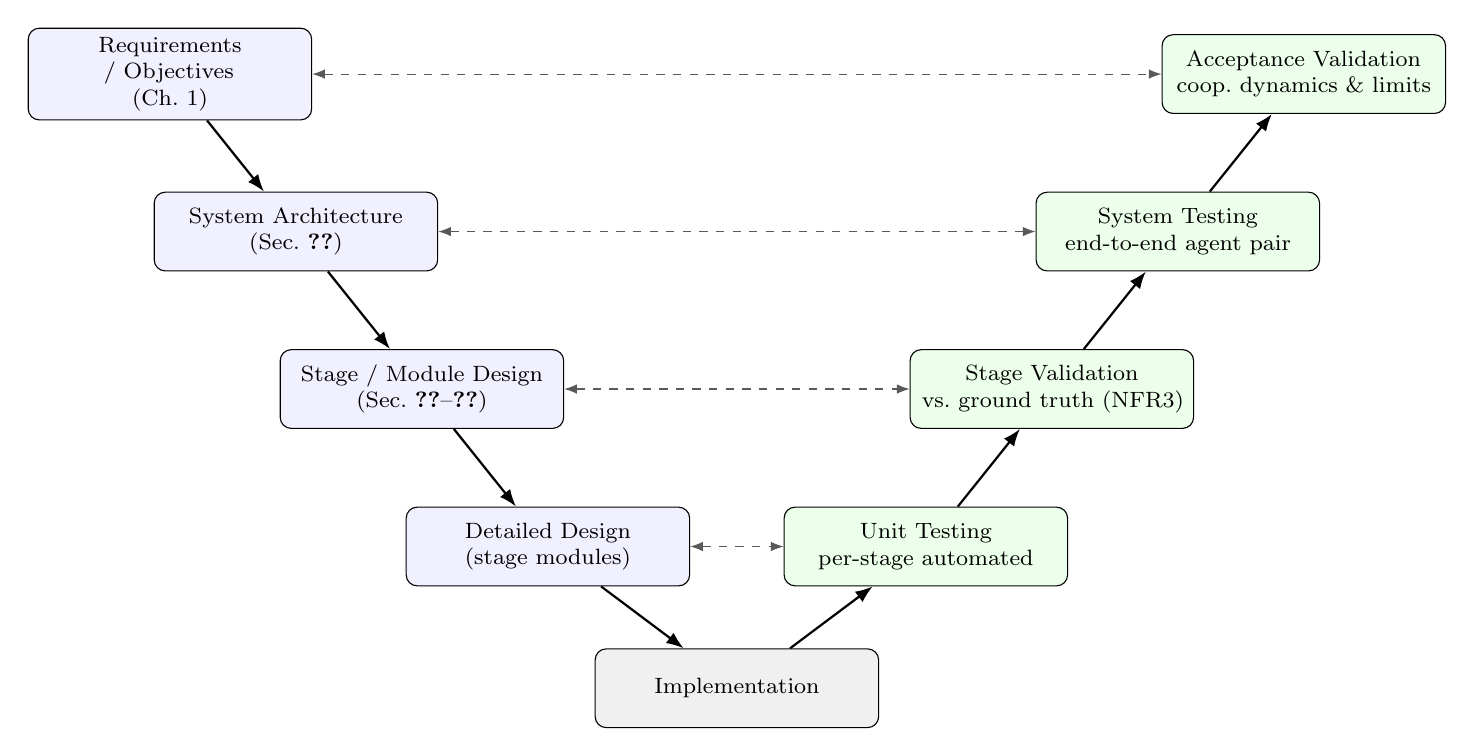
\begin{tikzpicture}[node distance=0pt,vbox/.append style={minimum width=3.6cm,text width=3.3cm}]
% Left (design) arm — descending
\node[vbox,fill=blue!6]   (L1) at (0,8)   {Requirements / Objectives\\\footnotesize(Ch.~1)};
\node[vbox,fill=blue!6]   (L2) at (1.6,6)  {System Architecture\\\footnotesize(Sec.~\ref{sec:architecture})};
\node[vbox,fill=blue!6]   (L3) at (3.2,4)  {Stage / Module Design\\\footnotesize(Sec.~\ref{sec:stage1}--\ref{sec:stage4})};
\node[vbox,fill=blue!6]   (L4) at (4.8,2)  {Detailed Design\\\footnotesize(stage modules)};
% Right (verification) arm — ascending
\node[vbox,fill=green!8]  (R1) at (14.4,8) {Acceptance Validation\\\footnotesize coop.\ dynamics \& limits};
\node[vbox,fill=green!8]  (R2) at (12.8,6) {System Testing\\\footnotesize end-to-end agent pair};
\node[vbox,fill=green!8]  (R3) at (11.2,4) {Stage Validation\\\footnotesize vs.\ ground truth (NFR3)};
\node[vbox,fill=green!8]  (R4) at (9.6,2)  {Unit Testing\\\footnotesize per-stage automated};
% Bottom vertex
\node[vbox,fill=gray!12]  (IM) at (7.2,0.2) {Implementation};
% V arms
\draw[flow] (L1) -- (L2); \draw[flow] (L2) -- (L3); \draw[flow] (L3) -- (L4); \draw[flow] (L4) -- (IM);
\draw[flow] (IM) -- (R4); \draw[flow] (R4) -- (R3); \draw[flow] (R3) -- (R2); \draw[flow] (R2) -- (R1);
% Horizontal correspondences
\draw[corr] (L1) -- (R1); \draw[corr] (L2) -- (R2); \draw[corr] (L3) -- (R3); \draw[corr] (L4) -- (R4);
\end{tikzpicture}}
\caption[The V-model as instantiated in this project]{The V-model as instantiated
in this project.}
\label{fig:vmodel}
\end{figure}

The horizontal correspondences are realized concretely in this project:

\begin{itemize}[leftmargin=*,itemsep=4pt]
  \item \textbf{Implementation $\leftrightarrow$ Unit testing.} Each stage is
  accompanied by an automated test module exercising its internal logic in isolation from the rest of the pipeline and from
  real data. These tests encode the detailed design contracts and are the first
  gate any change must pass.
  \item \textbf{Stage design $\leftrightarrow$ Stage validation.} Each stage has a
  dedicated, standalone validation procedure that scores its output against ground
  truth without invoking later stages (NFR3). This is the level at which a stage's
  design --- not just its code --- is confirmed to behave as intended on
  real inputs.
  \item \textbf{System architecture $\leftrightarrow$ System testing.} The
  architecture is exercised as a whole by running the complete chain --- depth,
  detection, lifting, and fusion --- for a genuine pair of cooperating agents,
  confirming that the stage interfaces compose correctly end to end.
  \item \textbf{Objectives $\leftrightarrow$ Acceptance validation.} The top-level
  question is answered by the final measurement of the cooperative gain in a
  controlled multi-agent setting, which is the engineering acceptance criterion for
  the thesis as a whole.
\end{itemize}

A practical consequence of this discipline is that defects are localized to the
narrowest possible level. A regression in a geometric routine surfaces at the unit
level; a degradation in depth quality surfaces at stage validation; an interface
mismatch surfaces at system testing. Because each level has an explicit owner in
the design, failures are diagnosed against the corresponding specification rather
than against the opaque end-to-end behaviour.

\section{System Architecture Overview}
\label{sec:architecture}

The proposed system is a \textbf{four-stage pipeline}. Each stage consumes the
output of its predecessor through a documented interface and emits artifacts that
are both the input to the next stage and an independently inspectable result. The
stages and their data interfaces are summarized in Table~\ref{tab:stages}, and their
end-to-end composition across a pair of cooperating vehicles is shown in
Figure~\ref{fig:pipeline}.

\begin{table}[htbp]
\centering
\caption{The four pipeline stages and their interfaces.}
\label{tab:stages}
\begin{tabularx}{\textwidth}{@{}clL@{}}
\toprule
\textbf{Stage} & \textbf{Name} & \textbf{Input $\rightarrow$ Output} \\
\midrule
1 & Depth  & Rectified stereo pair $\rightarrow$ dense disparity / metric depth \\
2 & Detect & Single (left) image $\rightarrow$ 2D vehicle regions \\
3 & Lift   & 2D regions + depth $\rightarrow$ 3D position per vehicle  \\
4 & Fuse & Two agents' 3D observations + relative pose $\rightarrow$ one fused, registered scene \\
\bottomrule
\end{tabularx}
\end{table}

Stages 1 through 3 constitute the \textbf{single-vehicle perception chain}: they
take one vehicle's raw stereo imagery and turn it into a set of 3D vehicle
positions expressed in that vehicle's own camera frame. Stage 4 is the
\textbf{cooperative layer}: it takes the perception output of two such vehicles and
the geometric relationship between them, and produces a single shared scene. The first three stages fulfill Objective~1 (the single-agent 3D localisation baseline); Stage 4 addresses Objective~2 (the decentralised object-level fusion layer); and the performance analysis of the combined, end-to-end system addresses Objective~3 (the empirical characterisation of cooperative localisation dynamics).


\begin{figure}[htbp]
\centering
\resizebox{\textwidth}{!}{%
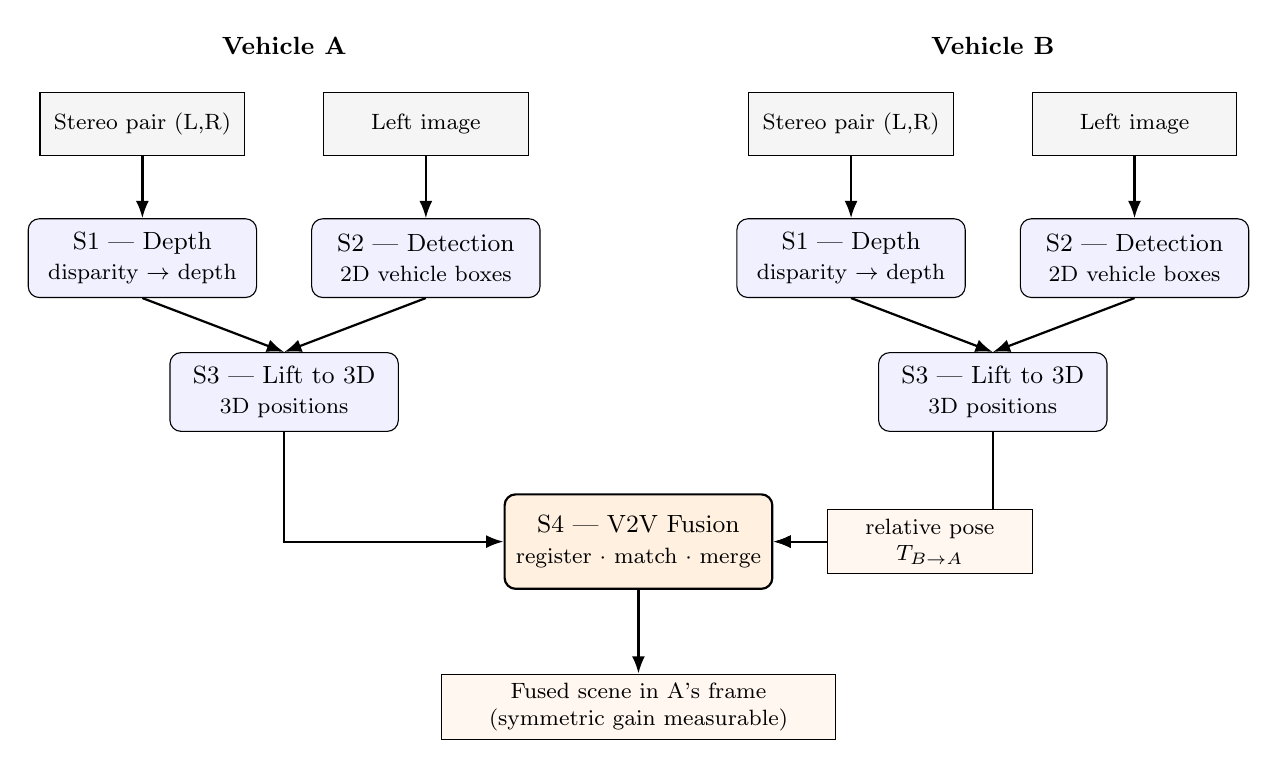
\begin{tikzpicture}[
  databox/.append style={minimum width=2.6cm},
  stagebox/.append style={minimum width=2.9cm},
  lbl/.style={font=\scriptsize,fill=gray!12,inner sep=1.5pt,rounded corners=1pt}]
% ---- Agent A : S1 (depth) and S2 (detection) run in parallel ----
\node[databox]  (srcA)  at (0,6)    {Stereo pair (L,R)};
\node[databox]  (imgA)  at (3.6,6)  {Left image};
\node[stagebox] (s1A)   at (0,4.3)  {S1 — Depth\\\footnotesize disparity $\rightarrow$ depth};
\node[stagebox] (s2A)   at (3.6,4.3){S2 — Detection\\\footnotesize 2D vehicle boxes};
\node[stagebox] (s3A)   at (1.8,2.6){S3 — Lift to 3D\\\footnotesize 3D positions};
\node[font=\bfseries\small] at (1.8,7) {Vehicle A};
% ---- Agent B (mirror) ----
\node[databox]  (srcB)  at (9,6)    {Stereo pair (L,R)};
\node[databox]  (imgB)  at (12.6,6) {Left image};
\node[stagebox] (s1B)   at (9,4.3)  {S1 — Depth\\\footnotesize disparity $\rightarrow$ depth};
\node[stagebox] (s2B)   at (12.6,4.3){S2 — Detection\\\footnotesize 2D vehicle boxes};
\node[stagebox] (s3B)   at (10.8,2.6){S3 — Lift to 3D\\\footnotesize 3D positions};
\node[font=\bfseries\small] at (10.8,7) {Vehicle B};
% ---- intra-agent flows ----
\foreach \s/\d in {srcA/s1A,imgA/s2A,srcB/s1B,imgB/s2B} \draw[flow] (\s) -- (\d);
\draw[flow] (s1A.south) -- (s3A.north) ;
\draw[flow] (s2A.south) -- (s3A.north) ;
\draw[flow] (s1B.south) -- (s3B.north) ;
\draw[flow] (s2B.south) -- (s3B.north) ;
% ---- fusion ----
\node[fusebox] (fus) at (6.3,0.7)
  {S4 — V2V Fusion\\\footnotesize register $\cdot$ match $\cdot$ merge};
\draw[flow] (s3A.south) |- (fus.west);
\draw[flow] (s3B.south) |- (fus.east);
\node[databox,fill=orange!6] (pose) at (10.0,0.7) {relative pose\\\footnotesize $T_{B\rightarrow A}$};
\draw[flow] (pose) -- (fus);
\node[databox,fill=orange!6,minimum width=5cm] (out) at (6.3,-1.4)
  {Fused scene in A's frame\\\footnotesize (symmetric gain measurable)};
\draw[flow] (fus) -- (out);
\end{tikzpicture}}
\caption[End-to-end data flow]{End-to-end data flow of the four-stage pipeline.}
\label{fig:pipeline}
\end{figure}

Two architectural properties follow from the requirements of
Section~\ref{sec:requirements} :

\begin{itemize}[leftmargin=*,itemsep=3pt]
  \item \textbf{Symmetry of the perception chain.} The identical Stage 1--3 chain
  is applied to each vehicle. Neither agent is privileged; cooperation is a
  relationship between two equal perception systems, which is what makes a
  symmetric benefit measurement (FR5) meaningful.
  \item \textbf{A single point of coupling.} The two perception chains are entirely
  independent until Stage 4. All inter-agent coupling is confined to the
  fusion layer, keeping the single-vehicle design free of cooperation-specific
  concerns.
\end{itemize}

\section{Data Sources and the Dual-Dataset Strategy}
\label{sec:data}

A recurring difficulty identified in Chapter~\ref{ch:introduction} is that no
single dataset offers both real stereo imagery and simultaneous
multi-vehicle recordings with trustworthy ground truth. The architecture resolves
this with a deliberate dual-dataset strategy, assigning each data source
the role it is uniquely suited to.

\begin{itemize}[leftmargin=*,itemsep=4pt]
  \item \textbf{Real-image stereo source (single-vehicle chain).} Stages 1--3 are
  designed and validated against real-world driving stereo data. This is the only
  way to confirm that the camera-only perception chain behaves on genuine imagery,
  with its real noise, lighting, and scene complexity. Because this source provides
  one vehicle's view at a time, it cannot exercise cooperation, but it is the
  authoritative ground for the single-vehicle claim.
  \item \textbf{Simultaneous multi-agent source (cooperative layer).} Stage 4
  requires two vehicles observing the same scene at the same instant,
  together with exact relative pose and a complete inventory of which objects each
  vehicle can truly see. These conditions are obtainable from a controlled
  simulation environment~\cite{dosovitskiy2017carla} that records two moving ego
  vehicles in a shared scene, with per-object, per-agent visibility derived from
  the rendered view rather than guessed geometrically. This source is what makes
  the cooperative gain measurable (FR5) with reliable ground truth.
\end{itemize}

This division is an engineering decision rather than a compromise: each stage is
exercised on the data that can actually test it. The shared
interface contract between the stages (Table~\ref{tab:stages}) is what allows the
same Stage 1--3 design to operate on either source.

\section{Stage 1 --- Stereo Depth Estimation}
\label{sec:stage1}

The remaining sections of this chapter make use of mathematical notation throughout. To keep them self-contained, the notation used is collected once in Appendix~\ref{app:notation} (Table~\ref{tab:notation}).

\paragraph{Purpose.} Stage 1 converts a rectified stereo image pair into a dense
estimate of per-pixel disparity, from which metric depth is recovered by the
standard stereo triangulation relationship~\cite{szeliski2022computer}
\begin{equation}
Z = \frac{f \cdot B}{d}
\label{eq:triangulation}
\end{equation}
where $Z$ is the depth of a pixel, $f$ the focal length in pixels, $B$ the stereo
baseline in metres, and $d$ the disparity (the horizontal displacement of the pixel
between the left and right images). The baseline itself is recovered from the two
cameras' projection matrices, $B = (t_x^{L} - t_x^{R}) / f$, where $t_x^{L}$ and
$t_x^{R}$ are the horizontal translation terms of the left and right projection
matrices.

This relationship is central to the entire methodology and reappears as the
dominant source of error analysed in later chapters. Differentiating it with
respect to disparity gives the depth error induced by a disparity error:
\begin{equation}
\left| \Delta Z \right| \;\approx\; \frac{Z^{2}}{f \cdot B}\, \left| \Delta d \right|
\label{eq:deptherror}
\end{equation}

Because the depth error scales with the square of the distance, a fixed
disparity error of a fraction of a pixel translates into a small error nearby but a
large one far away. The system is therefore expected, by construction, to be most
accurate on nearby vehicles --- a property that informs the design of every
subsequent stage and that is quantified empirically in Chapter~5.

\paragraph{Design.} The stage is built around two interchangeable depth estimators
that represent two distinct engineering trade-offs, selectable without altering any
downstream stage:

\begin{itemize}[leftmargin=*,itemsep=3pt]
  \item A \textbf{classical semi-global block-matching estimator}~\cite{hirschmuller2008},
  which produces a sparse disparity map: it reports depth only where a
  confident left--right correspondence exists and leaves textureless or ambiguous
  regions unfilled. Its sparsity is, in effect, a built-in reliability filter ---
  the pixels it does report tend to lie on well-defined surfaces.
  \item A \textbf{learned deep-stereo estimator}~\cite{wang2026}, which
  produces a dense disparity map with full coverage, at greater
  computational cost. It is run directly as an in-process inference step.
\end{itemize}

Offering both is a deliberate architectural choice. It allows the methodology to
separate questions of depth accuracy from questions of downstream
robustness: a sparse, conservative map and a dense, complete map stress the later
stages differently, and carrying both through the pipeline lets the project reason
about that trade-off rather than presuppose a single answer.

\paragraph{Interface.} The stage emits a per-pixel disparity map in which invalid
pixels are explicitly marked, so that downstream stages can distinguish ``no
measurement'' from ``a measurement of zero.'' This explicit invalid-pixel contract
is what allows the sparse and dense estimators to share one interface.

\section{Stage 2 --- 2D Object Detection}
\label{sec:stage2}

\paragraph{Purpose.} Stage 2 locates the surrounding vehicles in the (left) camera
image as two-dimensional regions. It answers where in the image the objects
of interest are, the question of where in space is addressed separately, in Stage 3.

\paragraph{Design.} The stage uses a pretrained transformer-based object
detector~\cite{lv2024} applied to the left image of the stereo pair. Detection
operates on the single image rather than on the depth map because appearance-based
detection is mature and robust, whereas the depth map is better used for
localizing an already-detected object than for finding it. The
detector is pretrained on a general-purpose object vocabulary; the stage maps the
relevant vehicle categories of that vocabulary onto the project's target class and
discards the rest, applying a confidence threshold to suppress weak detections.

\paragraph{Class scope.} The pipeline is deliberately scoped to a single object
class --- the car. Restricting the class keeps the evaluation interpretable and aligned
with the honesty principle (NFR4). The architecture does not preclude additional
classes; re-enabling them is a configuration concern localized to the detection and
matching stages.

\paragraph{Interface.} The stage emits, per image, a set of labelled 2D regions
with associated confidences, which become the input to the lifting stage alongside
the Stage 1 depth map.

\section{Stage 3 --- Lifting to 3D Position}
\label{sec:stage3}

\paragraph{Purpose.} Stage 3 is the junction of the two preceding stages: it
combines each 2D detection (Stage 2) with the depth map (Stage 1) and the camera
calibration to place the detected vehicle at a three-dimensional position in the
observing vehicle's camera frame. This is the stage at which the system crosses
from image space into the metric 3D world in which cooperation takes place.

\paragraph{The position-only design decision.} The single most important
methodological decision in the single-vehicle chain is that Stage 3 outputs 3D
position only --- a point $(x, y, z)$ per vehicle, carried together with the source
2D region --- and deliberately does not output a full 3D bounding box with
size and heading. This decision is a direct application of the honesty principle
(NFR4) and follows from the range-dependent stereo uncertainty at the heart of the
problem statement (Chapter~\ref{ch:introduction}).

The reasoning is geometric. Recovering an object's position requires
establishing how far away it is, which stereo supports. Recovering an object's
size and heading, by contrast, requires resolving its
three-dimensional extent and orientation from a single viewpoint at range --- and
the same disparity-to-depth sensitivity that limits position accuracy at distance
makes extent and orientation far less observable still. 

\paragraph{Design.} For each 2D region, the stage samples a representative depth
from the disparity map within the region, converts it to a metric distance via the
stereo relationship of Section~\ref{sec:stage1}, and unprojects the region's centre
to a 3D point using the camera calibration. All 3D quantities are expressed in the
KITTI camera convention ($X$ right, $Y$ down, $Z$ forward into the scene;
Figure~\ref{fig:frames}). Given a region centre at pixel $(u, v)$ and its sampled
depth $Z$, the inverse of the pinhole projection yields the 3D point
\begin{equation}
X = \frac{(u - c_x)\, Z}{f_x}, \qquad
Y = \frac{(v - c_y)\, Z}{f_y}, \qquad
Z = Z
\label{eq:unproject}
\end{equation}
where $(f_x, f_y)$ are the focal lengths and $(c_x, c_y)$ the principal point of the
left camera, both read from its calibration. The point $(X, Y, Z)$ is the vehicle's
position in the observing vehicle's camera frame. Two considerations shape this:

\begin{itemize}[leftmargin=*,itemsep=4pt]
  \item \textbf{Robust depth sampling within a region.} A detection's region
  contains pixels belonging to the vehicle but also, typically, road surface and
  background. The stage therefore does not take a naive average; it samples depth in
  a way designed to favour the object surface over contaminating background, with
  the sampling strategy tuned per depth estimator because the sparse and dense maps
  of Stage 1 have very different pixel distributions inside a region. The specific
  tuning is treated as an experimental matter and reported in Chapter~5.
  \item \textbf{Confidence propagation.} The 3D position inherits a confidence that
  scales the 2D detection confidence by the proportion of the region for which valid
  depth was available, $c_{3D} = c_{2D} \cdot \rho$, where the coverage ratio
  $\rho \in [0, 1]$ is the fraction of region pixels carrying a valid depth
  measurement. A position lifted from a well-covered region is thus trusted more
  than one lifted from a sparsely measured region, and this confidence later
  participates directly in the fusion merge (Section~\ref{sec:stage4}).
\end{itemize}

\paragraph{Interface.} The stage emits, per detected vehicle, a labelled 3D
position with its propagated confidence and the source 2D region. This compact,
position-only representation is intentionally schema-compatible with the fusion
core, which is designed to operate whether or not size and heading are present.

\section{Stage 4 --- Cooperative V2V Fusion}
\label{sec:stage4}

Stage 4 is the cooperative layer and the realization of the thesis goal. It takes
the independent 3D observations of two vehicles and combines them into a single
shared scene in which objects visible to either vehicle become known to both.
Combining detections after each vehicle has perceived independently is the
late fusion strategy for cooperative perception~\cite{xu2022opv2v}, chosen
here because it keeps the inter-vehicle interface compact (3D positions rather than
raw imagery) and the single-vehicle chain unaware of cooperation. Its design
separates a source-agnostic fusion core from the data plumbing that
feeds it, so that the same fusion logic operates on either real or simulated inputs
and on either position-only or fully-specified boxes.

The fusion proceeds in three conceptual steps --- \textbf{register, match, merge}
--- preceded by the construction of the common frame (Figure~\ref{fig:fusion}).

\paragraph{Common frame and registration.} Each vehicle perceives in its own camera
frame; the two frames are unrelated until the vehicles' relative pose is known.
Cooperation therefore begins by choosing one vehicle's frame (Vehicle A's) as the
reference and transforming the other vehicle's observations into it by a single
rigid $4\times4$ homogeneous transform derived from the two vehicles' poses,
\begin{equation}
T_{B \rightarrow A} = M \; T_{W,A}^{-1} \; T_{W,B} \; M^{-1}
\label{eq:registration}
\end{equation}
where $T_{W,A}$ and $T_{W,B}$ are the world-from-camera transforms of the two
vehicles (each built from the vehicle's world pose composed with its fixed camera
mount), and $M$ is the constant axis map from the vehicle frame to the KITTI camera
convention, $(x, y, z)_{\text{cam}} = (y, -z, x)_{\text{vehicle}}$
(Figure~\ref{fig:frames}). Any 3D point observed by Vehicle B is then carried into
A's frame by $\tilde{p}_A = T_{B \rightarrow A}\, \tilde{p}_B$ (in homogeneous
coordinates), and a box's heading is offset by the transform's rotation about the
camera vertical axis, $\theta_{\text{offset}} = \operatorname{atan2}(R_{13}, R_{33})$,
extracted from the rotation block $R$ of $T_{B \rightarrow A}$. Because the
cooperative source records simultaneous observations, this is a purely spatial
alignment --- there is no temporal extrapolation, and a static object seen by both
vehicles should, after registration, coincide. The design exploits exactly this
property as a built-in correctness check: an object seen by both agents must
register to near-zero displacement, and a large displacement is treated as a symptom
of a coordinate or pose error rather than of a moving object. This sanity check is
part of the methodology: it is the mechanism by which the
most dangerous class of bug in cooperative perception, a silent frame misalignment,
is caught.

\begin{figure}[htbp]
\centering
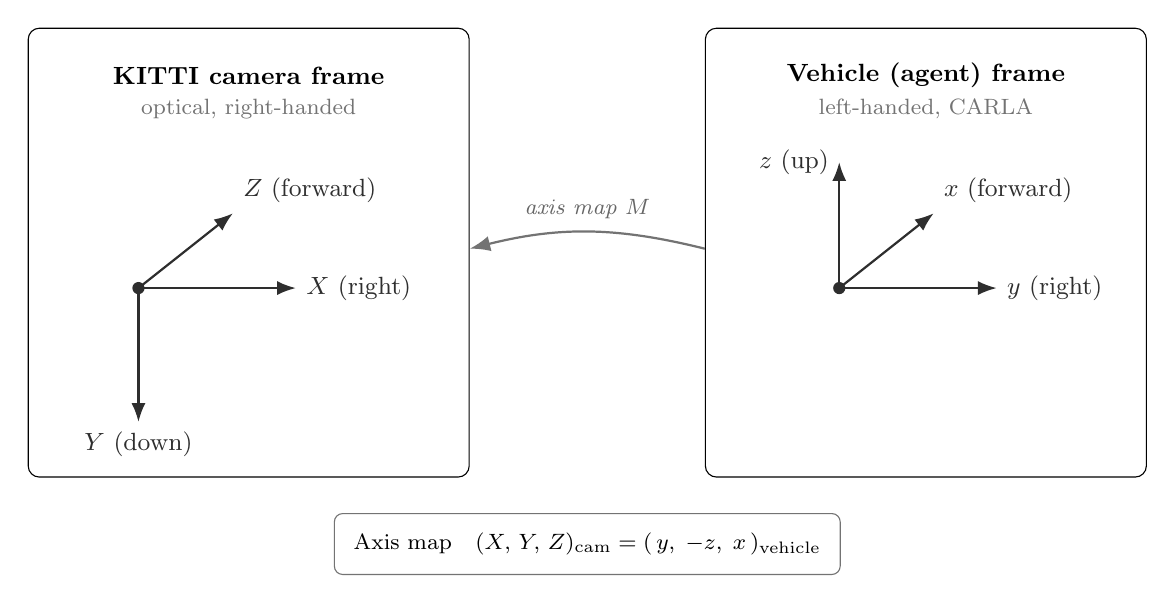
\begin{tikzpicture}[
    >={Latex[length=2.4mm]},
    axis/.style={->,thick,black!82},
    ttl/.style={font=\bfseries\small,align=center},
    sub/.style={font=\footnotesize,text=black!55,align=center},
    alab/.style={font=\small},
    panel/.style={draw=black,rounded corners=4pt,minimum width=5.6cm,minimum height=5.7cm}]
% ===== equal-size frames (black border, no fill) =====
\begin{scope}[on background layer]
  \node[panel] (cpan) at (1.4,0.45) {};
  \node[panel] (vpan) at (10.0,0.45) {};
\end{scope}
% ===== KITTI camera frame axes =====
\coordinate (oc) at (0,0);
\draw[axis] (oc) -- (2.0,0)    node[alab,right]      {$X$ (right)};
\draw[axis] (oc) -- (0,-1.7)   node[alab,below]      {$Y$ (down)};
\draw[axis] (oc) -- (1.2,0.95) node[alab,above right]{$Z$ (forward)};
\fill[black!82] (oc) circle (2.2pt);
\node[ttl] at (1.4,2.7)  {KITTI camera frame};
\node[sub] at (1.4,2.28) {optical, right-handed};
% ===== Vehicle frame axes =====
\coordinate (ov) at (8.9,0);
\draw[axis] (ov) -- ($(ov)+(1.2,0.95)$) node[alab,above right]{$x$ (forward)};
\draw[axis] (ov) -- ($(ov)+(2.0,0)$)    node[alab,right]      {$y$ (right)};
\draw[axis] (ov) -- ($(ov)+(0,1.6)$)    node[alab,left]       {$z$ (up)};
\fill[black!82] (ov) circle (2.2pt);
\node[ttl] at (10.0,2.7)  {Vehicle (agent) frame};
\node[sub] at (10.0,2.28) {left-handed, CARLA};
% ===== axis-map bridge arrow, in the gap between the two boxes =====
\coordinate (mid) at (0,0.5);
\draw[-{Latex[length=2.6mm]},thick,black!55]
  (vpan.west |- mid) to[bend right=14]
  node[above=1pt,font=\footnotesize\itshape,text=black!60]{axis map $M$}
  (cpan.east |- mid);
% ===== axis-map equation, centred under the whole figure =====
\node[draw=black!55,rounded corners=3pt,fill=none,font=\footnotesize,inner sep=7pt,anchor=north]
  at ([yshift=-0.45cm]current bounding box.south)
  {Axis map\quad $(X,\,Y,\,Z)_{\text{cam}} = (\,y,\; -z,\; x\,)_{\text{vehicle}}$};
\end{tikzpicture}
\caption[The two coordinate frames]{Spatial Mapping Between KITTI Optical and CARLA Vehicle Coordinate Frames}
\label{fig:frames}
\end{figure}

\paragraph{Matching.} Registered observations from the two vehicles are associated
greedily by bird's-eye-view (ground-plane) centre distance, within object class,
accepting a pair as the same physical object only when their separation falls below
a per-class threshold $\tau$. The bird's-eye-view distance discards the vertical
axis and measures separation in the ground plane,
\begin{equation}
d_{\text{BEV}}(a, b) = \sqrt{(x_a - x_b)^2 + (z_a - z_b)^2}, \qquad
\text{match if } d_{\text{BEV}} \le \tau
\label{eq:bev}
\end{equation}
candidate pairs being considered in ascending order of distance so that the closest
compatible pair is committed first. Matching on ground-plane centre distance ---
rather than on 3D box overlap --- is the natural choice given the position-only
output of Stage 3, and it is exactly what makes the fusion core able to consume both
position-only and fully-specified inputs through one code path.

\paragraph{Merge.} A corroborated pair --- one object that both vehicles saw --- is
merged into a single estimate. Writing the two observations' confidences as $c_A$
and $c_B$, each merged position coordinate is the confidence-weighted average of the
two observations, and the fused confidence is combined by a noisy-OR rule:
\begin{equation}
\hat{x} = \frac{c_A\, x_A + c_B\, x_B}{c_A + c_B}
\quad (\text{and likewise for } y, z), \qquad
\hat{c} = 1 - (1 - c_A)(1 - c_B)
\label{eq:merge}
\end{equation}
The noisy-OR rule reflects that two independent detections of the same object are
more trustworthy than either alone (the fused confidence exceeds both inputs). Where
the inputs happen to carry size and heading, those are merged too --- dimensions by
the same confidence-weighted average, and heading by a confidence-weighted
\emph{circular} mean,
\begin{equation}
\hat{\theta} = \operatorname{atan2}\!\Big(\textstyle\sum_i c_i \sin\theta_i,\; \sum_i c_i \cos\theta_i\Big),
\label{eq:circmean}
\end{equation}
which averages angles correctly across the $\pm\pi$ wrap-around. The merge is
nonetheless designed to degrade gracefully to position-only when size and heading
are absent. An object seen by only one vehicle is carried into the shared scene
unmerged, tagged with its source --- this is precisely the blind-spot recovery that
motivates the whole system. A matched pair whose post-registration displacement is
implausibly large is not merged but flagged, on the principle that for
simultaneous observations a large displacement indicates a faulty match or pose
error rather than genuine motion.

\begin{figure}[H]
\centering
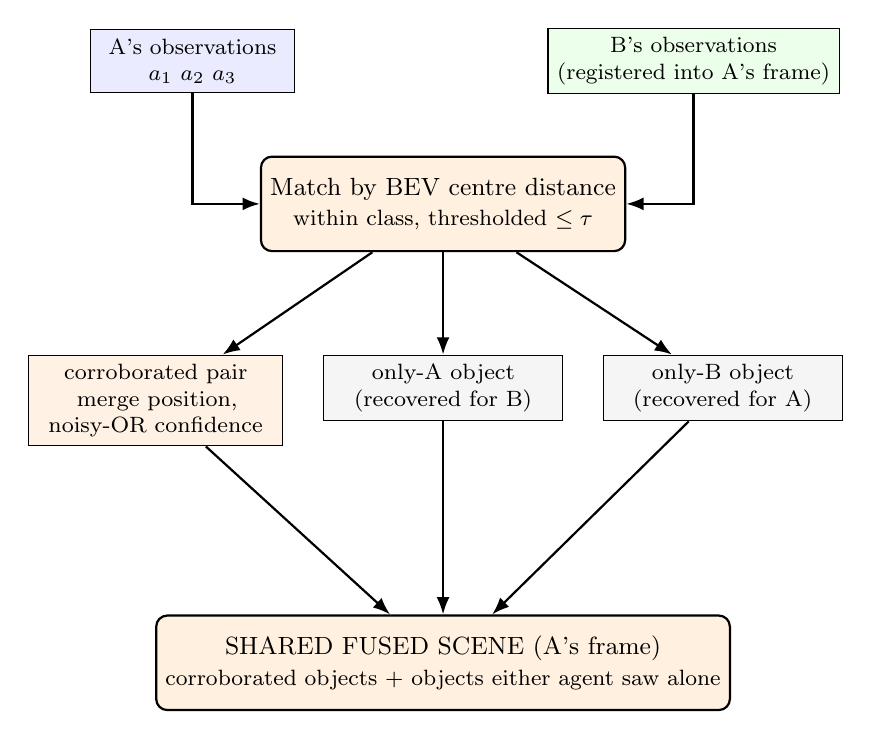
\begin{tikzpicture}[node distance=0.6cm and 1.2cm]
\node[databox,fill=blue!8] (a) {A's observations\\\footnotesize $a_1\ a_2\ a_3$};
\node[databox,fill=green!8,right=3.2cm of a] (b)
  {B's observations\\\footnotesize (registered into A's frame)};
\node[fusebox,below=1.2cm of {$(a)!0.5!(b)$},minimum width=4.4cm] (match)
  {Match by BEV centre distance\\\footnotesize within class, thresholded $\le \tau$};
\draw[flow] (a.south) |- (match.west);
\draw[flow] (b.south) |- (match.east);
% outcomes
\node[databox,below left=1.3cm and -0.3cm of match,fill=orange!10,text width=3.0cm] (corr)
  {corroborated pair\\\footnotesize merge position,\\ noisy-OR confidence};
\node[databox,below=1.3cm of match,fill=gray!8,text width=2.8cm] (onlyA)
  {only-A object\\\footnotesize (recovered for B)};
\node[databox,below right=1.3cm and -0.3cm of match,fill=gray!8,text width=2.8cm] (onlyB)
  {only-B object\\\footnotesize (recovered for A)};
\foreach \n in {corr,onlyA,onlyB} \draw[flow] (match) -- (\n);
\node[fusebox,below=4.6cm of match,minimum width=6.2cm,fill=orange!12] (scene)
  {SHARED FUSED SCENE (A's frame)\\\footnotesize corroborated objects $+$ objects either agent saw alone};
\foreach \n in {corr,onlyA,onlyB} \draw[flow] (\n) -- (scene);
\end{tikzpicture}
\caption[The register--match--merge logic of the fusion core]{The
register--match--merge logic of the fusion core.}
\label{fig:fusion}
\end{figure}

\paragraph{Symmetric benefit by design.} The fused output is a single shared
scene, and this is what allows the cooperative benefit to be measured symmetrically
(FR5). Evaluation is framed against a cooperative ground truth --- the union
of every object visible to either vehicle, de-duplicated by object identity --- and
the shared scene is scored from both vehicles' standpoints: how many objects each
vehicle recovered that it could not have seen alone, and whether its localization of
objects it could see improved. The architecture treats the two vehicles identically
in this accounting, so neither agent's gain is privileged. Because the two ego
vehicles are themselves part of the simulated scene yet are not perception
targets (their poses are shared directly over the cooperative link), the
evaluation design treats an agent's detection of the other ego as neither a
hit nor a false alarm --- an ignore region --- so that the cooperation metric
reflects perceived traffic rather than the agents perceiving each other.

\bigskip
\noindent Two design commitments give the framework its character. The first is honesty
about sensing limits: because stereo cannot reliably recover object size or heading
at range, the system outputs 3D position only, and structures both its
representation and its evaluation around what cameras can actually provide. The
second is verification by construction: the V-model pairs every level of
design with the level of testing that confirms it, so that the headline cooperative
result rests on independently validated stages rather than on end-to-end behaviour
alone. With the architecture and process established, Chapter~4 details the
experimental setup and simulation environment, and Chapter~5 reports the stagewise
validation and the characterisation of the cooperative localisation dynamics that
this framework was built to measure.

\chapter{Experimental Setup and Simulation Environment}
\label{ch:experimental}

Chapter~\ref{ch:methodology} presented the architecture of the four-stage pipeline
and the V-model discipline under which it was built. This chapter specifies the
conditions under which that pipeline is exercised and measured: the datasets that
feed it, the simulation environment that supplies simultaneous multi-agent ground
truth, the concrete model and algorithm configurations of each stage, and the
evaluation metrics against which every stage is scored. The results obtained under
this setup are reported and discussed in Chapter~5; the present chapter establishes
\emph{what} is measured and \emph{how}, so that those results are reproducible and
interpretable.

The experimental design is a direct consequence of the dual-dataset strategy of
Section~\ref{sec:data}. The single-vehicle perception chain (Stages~1--3) is
exercised on real driving imagery from the KITTI benchmark suite, the only source
that can confirm camera-only perception on genuine sensor data. The cooperative
layer (Stage~4) is exercised on the CARLA simulator, the source that can provide
two vehicles observing one scene at one instant with exact relative pose and
occlusion-truthful per-agent visibility. Each dataset is described in the role it
serves, followed by the per-stage configurations and the metric definitions.

\section{Implementation and Software Environment}
\label{sec:environment}

The pipeline is implemented in Python, with each stage as a standalone, command-line
runnable module that communicates with its neighbours only through on-disk artifacts
(disparity maps, detection files, lifted-position files), consistent with the
modularity requirement (NFR1). The principal third-party components are OpenCV
(classical stereo matching and image I/O), PyTorch and the HuggingFace Transformers
library (the learned depth and detection models), NumPy and Shapely (geometry), and
MLflow (experiment tracking).

Two cross-cutting properties of the environment are essential to the validity of the
reported results:

\begin{itemize}[leftmargin=*,itemsep=3pt]
  \item \textbf{Determinism.} The random seeds of the \texttt{random}, NumPy, and
  PyTorch libraries are fixed to $42$ at every entry point. Combined with the
  configuration-driven design --- every operational value (paths, thresholds, model
  choices, tuned parameters) lives in a per-stage YAML configuration file rather
  than in code --- this makes each run reproducible from its recorded configuration
  (NFR2).
  \item \textbf{Experiment tracking.} Every run logs its parameters and resulting
  metrics to a persistent MLflow store, so that no result exists only as transient
  console output and any reported figure can be traced back to the run that produced
  it.
\end{itemize}

All experiments in this work were run on \textbf{CPU only}, with no GPU
acceleration. This constraint is itself a meaningful part of the setup: it reflects
the cost-constrained, camera-based deployment scenario motivating the thesis, and it
directly shapes the runtime trade-off between the classical and learned depth
estimators discussed in Section~\ref{sec:stage1cfg}.

\section{Real-Image Stereo Dataset: KITTI}
\label{sec:kitti}

The single-vehicle chain is developed and validated on the KITTI vision benchmark
suite~\cite{geiger2012kitti}, a standard real-world autonomous-driving dataset
recorded from a stereo camera rig mounted on a moving vehicle. Two of its splits are
used, each matched to the stages it can validate.

\subsection{Object split (Stages 1--2)}

The object detection split provides individual stereo frames with rectified
left/right images, per-frame camera calibration, dense disparity ground truth, and
labelled 2D object boxes. It is used to validate Stage~1 (depth) and Stage~2 (2D
detection) in isolation. The validation reported in Chapter~5 uses the first ten
frames of the split (\texttt{000000}--\texttt{000009}); the disparity ground truth
of this split is what makes a direct, per-pixel depth-accuracy measurement possible.

\subsection{Tracking split (Stage 3)}

Validating the lifting stage requires \emph{3D} ground truth --- the true metric
position of each vehicle --- which the object split does not align with its stereo
frames. Stage~3 is therefore validated on the KITTI tracking split, whose sequences
carry per-frame 3D object labels registered to the camera frame. The Stage~3
evaluation in Chapter~5 uses five sequences (24 frames in total). Each 2D detection
is lifted to a 3D position and compared against the tracking labels by 3D centre
distance (Section~\ref{sec:metricslift}).

\begin{table}[htbp]
\centering
\caption{KITTI conventions adopted by the pipeline.}
\label{tab:kitti}
\renewcommand{\arraystretch}{1.3}
\begin{tabularx}{\textwidth}{@{}lL@{}}
\toprule
\textbf{Item} & \textbf{Convention} \\
\midrule
Calibration keys & \texttt{P2}, \texttt{P3} (left/right projection matrices), \texttt{R\_rect\_00}, \texttt{Tr\_velo\_to\_cam} \\
Stereo baseline  & recovered as $B = (t_x^{L} - t_x^{R})/f$ from \texttt{P2}/\texttt{P3} \\
Disparity ground truth & 16-bit PNG; metric disparity $= \text{raw}/256.0$; $\text{raw}=0$ marks an invalid (no-measurement) pixel \\
Object vertical reference & label $y$ is the \emph{bottom} of the object (centre $= y - h/2$) \\
Coordinate frame & camera optical frame: $X$ right, $Y$ down, $Z$ forward \\
\bottomrule
\end{tabularx}
\end{table}

\subsection{KITTI conventions}

The pipeline adopts the standard KITTI conventions summarised in
Table~\ref{tab:kitti}. Of particular note for the depth and lifting stages: the
disparity ground truth is stored as a 16-bit image scaled by $256$, with a raw value
of zero denoting ``no measurement'' rather than zero disparity --- the explicit
invalid-pixel contract that Stage~1 preserves so that downstream stages never
mistake an absent measurement for a near-infinite depth.

\section{Simultaneous Multi-Agent Dataset: CARLA}
\label{sec:carla}

The cooperative layer cannot be validated on KITTI, which records only one vehicle's
view at a time. Stage~4 is therefore exercised on data generated with the CARLA
simulator~\cite{dosovitskiy2017carla}, which can render two vehicles observing the
same scene at the same instant with exact, noise-free relative pose --- and,
crucially, with per-object, per-agent visibility derived from the rendered view
rather than guessed geometrically.

\subsection{Scenario}

The scenario is a single urban intersection (the CARLA \texttt{Town10HD} map)
recorded over 300 synchronised frames, populated with traffic and two moving ego
vehicles. The two egos form a \textbf{leader--follower} pair: Vehicle~A travels close
to the shared traffic (median distance to the co-observed cars $\approx$~11~m) while
Vehicle~B follows roughly $3.3\times$ further behind (median $\approx$~36~m). This
geometry is deliberate --- it places the same vehicles at very different ranges from
the two agents, which is exactly the heterogeneous-uncertainty condition the thesis
sets out to study, and it furnishes a population of cars that the follower cannot
perceive alone, i.e.\ the blind-spot recovery that cooperation is meant to address.

\subsection{Per-agent recordings and data layout}

Each of the two agents (\texttt{vehicle\_a}, \texttt{vehicle\_b}) contributes, per
frame, a rectified stereo pair (\texttt{image\_left}/\texttt{image\_right}), a camera
calibration (\texttt{calib.json}), a noise-free disparity reference
(\texttt{disp\_noc\_0}), and its world pose (\texttt{pose.json}). A separate
per-frame ground-truth record (\texttt{gt\_boxes}) lists every vehicle in the scene
with its 3D box and the visibility metadata described below. This layout lets the
same Stage~1--3 chain that runs on KITTI run unchanged on each CARLA agent (the
detector path), after which Stage~4 fuses the two agents' outputs using the relative
pose derived from the two \texttt{pose.json} files.

\subsection{Visibility-truthful per-agent and cooperative ground truth}
\label{sec:coopgt}

The defining property of this dataset is that an object's visibility to each agent is
\emph{occlusion-truthful}. Each ground-truth box carries the number of its pixels
actually rendered to each agent's camera; a car counts as seen by an agent only if at
least \texttt{min\_visible\_pixels} ($=10$) of its pixels are visible to that agent.
Cars hidden behind buildings or other vehicles therefore correctly drop out of an
agent's truth set --- a geometric field-of-view test would have falsely credited an
agent with seeing them and thereby understated the cooperative benefit.

From these per-agent truth sets the \textbf{cooperative ground truth} is formed as
the union of every (non-ego) vehicle visible to A \emph{or} B, de-duplicated by
object identity (\texttt{actor\_id}). The two ego vehicles are part of the scene but
are not perception targets --- their poses are shared directly over the cooperative
link --- so they are excluded from the cooperative ground truth, and an agent's
detection of the \emph{other} ego is treated as an \textbf{ignore region} (neither a
true nor a false positive). Over the 150 frames evaluated in Chapter~5, the
cooperative ground truth comprises 9 distinct cars across 586 visible instances.

\section{Model and Algorithm Configurations}
\label{sec:configs}

Each stage is governed by a per-stage YAML configuration. The settings that
materially affect the results are summarised here; the full files are part of the
codebase.

\subsection{Stage 1 --- depth estimation}
\label{sec:stage1cfg}

The two interchangeable estimators of Section~\ref{sec:stage1} are configured as
follows. The classical estimator is OpenCV Semi-Global Block
Matching~\cite{hirschmuller2008} with a 192-pixel disparity search range, an
$11\times11$ matching block, smoothness penalties $P_1=8$ / $P_2=32$, a left--right
consistency check (\texttt{disp12\_max\_diff}~$=1$), a uniqueness ratio of $10\%$,
and speckle filtering --- a configuration that yields a \emph{sparse} but
consistency-checked disparity map. The smoothness penalties are kept intentionally
low because KITTI scenes have sharp depth discontinuities at object boundaries that
high penalties would over-smooth. The learned estimator is
WAFT-Stereo~\cite{wang2026}, run as an in-process inference step from a pretrained
checkpoint, producing a \emph{dense} (full-coverage) disparity map. On the CPU-only
environment of Section~\ref{sec:environment} the two differ sharply in cost ---
SGBM runs in the order of a second per image, WAFT in the order of a minute --- a
trade-off that is itself part of the analysis.

\subsection{Stage 2 --- 2D detection}

Detection uses RT-DETR~\cite{lv2024} (the \texttt{rtdetr\_r50vd} checkpoint,
$\approx$~43\,M parameters) applied to the left image, pretrained on the COCO object
vocabulary. The relevant COCO vehicle categories are remapped onto the project's
single target class --- \texttt{car}, \texttt{truck}, and \texttt{bus} all map to
KITTI \texttt{Car} --- and all other categories are discarded. A confidence
threshold of $0.5$ suppresses weak detections. Consistent with the Car-only scoping
of Section~\ref{sec:stage2}, no pedestrian or cyclist classes are emitted.

\subsection{Stage 3 --- lifting}

Lifting applies the per-method depth-sampling strategy motivated in
Section~\ref{sec:stage3}: for the sparse SGBM map, the $20^{\text{th}}$ percentile of
valid depths within a detection region with no vertical crop; for the dense WAFT map,
the $35^{\text{th}}$ percentile over the top $40\%$ of the box with depths nearer than
6~m gated out as road surface. A detection with fewer than 10 valid depth pixels in
its region is skipped rather than lifted from an empty frustum. These values are a
single source of truth in the Stage~3 configuration, read identically by the
pipeline and its validator.

\subsection{Stage 4 --- cooperative fusion}

Fusion matches A's observations against B's (registered into A's frame) greedily by
bird's-eye-view centre distance within class, accepting a pair as the same object
when their separation is at most $\tau_{\text{Car}}=2.0$~m. A matched pair is fused
only if its post-registration BEV displacement is below 1.0~m; a larger displacement
signals a faulty match or pose error (not motion, since the observations are
simultaneous) and the pair is flagged and kept unmerged. Fused confidence follows the
noisy-OR rule and fused position the confidence-weighted average of
Section~\ref{sec:stage4}.

\begin{table}[htbp]
\centering
\caption{Summary of the per-stage experimental configuration.}
\label{tab:configsummary}
\renewcommand{\arraystretch}{1.3}
\begin{tabularx}{\textwidth}{@{}llL@{}}
\toprule
\textbf{Stage} & \textbf{Component} & \textbf{Key settings} \\
\midrule
1 & SGBM / WAFT-Stereo & 192-px range, $11\times11$ block, $P_1/P_2=8/32$, LR-check / pretrained dense model \\
2 & RT-DETR (\texttt{r50vd}) & COCO $\rightarrow$ Car (car/truck/bus), confidence $\ge 0.5$ \\
3 & Lift-to-position & SGBM: p20, no crop; WAFT: p35, top-40\% crop, 6\,m gate; skip $<10$ px \\
4 & Late fusion & BEV match $\tau_{\text{Car}}=2.0$\,m, fuse if displacement $<1.0$\,m, noisy-OR confidence \\
\bottomrule
\end{tabularx}
\end{table}

\section{Evaluation Metrics}
\label{sec:metrics}

Each stage is scored against ground truth in isolation, so that a failure at any
level can be diagnosed without trusting its successors (NFR3). The metrics for each
stage are defined below.

\subsection{Stage 1 --- depth}

Disparity quality is measured against the dense ground-truth disparity, over valid
pixels only, by two standard KITTI metrics and a coverage figure:

\begin{itemize}[leftmargin=*,itemsep=3pt]
  \item \textbf{End-Point Error (EPE)} --- the mean absolute disparity error in
  pixels, $\text{EPE} = \frac{1}{N}\sum_i |d_i - d_i^{\text{GT}}|$.
  \item \textbf{D1 error} --- the percentage of pixels whose disparity error exceeds
  the standard KITTI outlier threshold (3~px and $5\%$ of the true disparity),
  capturing gross mismatches rather than sub-pixel noise.
  \item \textbf{Coverage} --- the percentage of pixels for which the estimator
  reports a valid disparity. This distinguishes the sparse SGBM map from the dense
  WAFT map and is essential context for the two preceding metrics, which are computed
  over reported pixels only.
\end{itemize}

\subsection{Stage 2 --- 2D detection}

Detection is scored by the standard average-precision framework. A predicted box is a
true positive when its Intersection-over-Union (IoU) with a ground-truth box of the
same class exceeds $0.5$. Per-class Average Precision (AP) and the mean over classes
(mAP) are reported, together with per-class precision and recall at the fixed
operating confidence threshold of $0.5$. Average precision is computed by 11-point
interpolation; a reliability flag marks evaluations made on fewer than ten frames as
small-sample estimates.

\subsection{Stage 3 --- lifting to 3D position}
\label{sec:metricslift}

Because Stage~3 emits a 3D \emph{position} plus the source 2D box --- not a full 3D
box --- it cannot be scored by 3D IoU. Instead a predicted position is matched to the
nearest unmatched same-class ground-truth object within a 3D centre-distance
threshold (Car~$\le 2.0$~m), greedily. From the resulting matches the pipeline
reports precision, recall, and their harmonic mean $F_1$, alongside two localisation
errors averaged over matched pairs: the \textbf{depth error} (error along the camera
forward axis $Z$) and the \textbf{3D centre distance}. To expose the central
range-dependence claim of Chapter~\ref{ch:introduction}, errors are additionally
broken down into depth-range bins (0--10, 10--20, 20--40, and beyond~40~m).

\subsection{Stage 4 --- cooperative fusion}
\label{sec:metricsfusion}

Stage~4 is evaluated against the cooperative ground truth of
Section~\ref{sec:coopgt}. For each frame, three prediction sets are scored against
the \emph{same} cooperative ground truth: \textbf{A-alone}, \textbf{B-alone} (B's
single-vehicle output registered into A's frame), and \textbf{Fused}. Each set is
matched to the cooperative ground truth by the same greedy BEV centre-distance rule
($\tau_{\text{Car}}=2.0$~m), giving per-set precision, recall, and a bird's-eye-view
\textbf{localisation error} over true positives. Beyond these per-set figures, the
following metrics characterise the cooperation itself:

\begin{itemize}[leftmargin=*,itemsep=3pt]
  \item \textbf{Symmetric cooperative gain.} Because the fused scene is shared, the
  benefit is measured for both agents against the same ground truth: A's gain from B
  is the set of cooperative-GT objects only B saw (\texttt{b\_unique\_tp}), and B's
  gain from A is the set only A saw (\texttt{a\_unique\_tp}), each reported as a
  recall improvement and a count of recovered objects.
  \item \textbf{Corroboration rate.} Of the objects co-observed by both agents, the
  fraction that are actually merged into a single fused estimate (as opposed to
  surviving as two separate detections). This distinguishes a genuinely
  deduplicated scene from one that is merely a union of the two agents' detections.
  \item \textbf{Angular separation.} The angle subtended at a co-observed car between
  the two agents' viewing directions, reported as a diagnostic for whether
  cross-view triangulation (which would tighten depth) is geometrically available.
  \item \textbf{Precision--recall sweep and localisation-vs-range curve.} A PR sweep
  over the confidence threshold traces the precision/recall trade-off of the three
  sets, and a plot of localisation error against ground-truth range exposes how the
  cooperative localisation behaves as targets recede.
\end{itemize}

\section{Experimental Protocol and Scope}
\label{sec:protocol}

The protocol follows directly from the V-model verification strategy: each stage is
run and scored standalone against the ground truth of the dataset best able to test
it, and only then is the full chain run end-to-end for a cooperating pair. Throughout,
the two depth estimators (SGBM and WAFT-Stereo) are carried through the entire
pipeline in parallel, so that the influence of depth density and accuracy on every
downstream stage --- detection-independent lifting quality and, ultimately,
cooperative recall and localisation --- can be attributed rather than presupposed.

Two scope conditions bound the interpretation of the results in Chapter~5 and are
stated here in the interest of honesty about what the setup can and cannot establish.
First, the cooperative evaluation rests on a \emph{single} scenario --- one
\texttt{Town10HD} intersection with a leader--follower pair and nine Car-only
cooperative-GT vehicles within 40~m --- so it is a characterised feasibility study,
not a multi-scenario benchmark. Second, the leader--follower geometry fixes the two
agents at a narrow angular separation from the shared cars; testing the
triangulation regime, in which two near-perpendicular viewpoints could tighten depth,
would require a different scenario geometry. These conditions do not weaken the
measurement; they delimit precisely the operating regime within which it is valid.

\bigskip
\noindent This chapter has specified the experimental setup: a deterministic, CPU-only,
configuration-driven, MLflow-tracked implementation; the KITTI benchmark suite as the
real-image source for the single-vehicle chain (object split for depth and detection,
tracking split for lifting); the CARLA \texttt{Town10HD} leader--follower scenario as
the simultaneous, occlusion-truthful multi-agent source for cooperative fusion; the
concrete per-stage model and algorithm configurations; and the metric definitions
against which each stage is scored, from per-pixel disparity error through cooperative
recall, localisation, and corroboration. With the setup established, Chapter~5
presents the stagewise validation results and the characterisation of the cooperative
localisation dynamics that this framework was built to measure.


% ------------------------------ Appendices ------------------------------------
\appendix
\chapter{Notation}
\label{app:notation}

This appendix collects the notation used throughout the methodology
(Chapter~\ref{ch:methodology}, Sections~\ref{sec:stage1}--\ref{sec:stage4}).

\begin{table}[htbp]
\centering
\caption{Notation used throughout the methodology (Sections~\ref{sec:stage1}--\ref{sec:stage4}).}
\label{tab:notation}
\begin{tabularx}{\textwidth}{@{}lL@{}}
\toprule
\textbf{Symbol} & \textbf{Meaning} \\
\midrule
$f,\; B,\; d$ & focal length (px), stereo baseline (m), disparity (px) \\
$Z$ & depth $=$ camera-frame forward coordinate (m) \\
$(u, v)$ & pixel coordinates in the image \\
$f_x, f_y$ & camera focal lengths along the image axes (px); $f_x \equiv f$ \\
$(c_x, c_y)$ & principal point of the left camera (px) \\
$(X, Y, Z)$ & 3D point in the camera frame (m): $X$ right, $Y$ down, $Z$ forward \\
$\rho$ & depth coverage ratio of a detection region, $\rho \in [0, 1]$ \\
$c_{2D},\; c_{3D}$ & 2D-detection confidence and propagated 3D confidence \\
$c_A, c_B,\; \hat{c}$ & the two agents' confidences and the fused confidence \\
$\tau$ & per-class BEV matching distance threshold (m) \\
$d_{\text{BEV}}$ & bird's-eye-view (ground-plane) centre distance (m) \\
$T_{W,A},\; T_{W,B}$ & world-from-camera transforms of Vehicles A and B ($4\times4$) \\
$T_{B \rightarrow A}$ & rigid transform mapping B's camera frame into A's ($4\times4$) \\
$M$ & fixed axis map from the vehicle frame to the camera frame \\
$R$ & rotation ($3\times3$) block of a homogeneous transform \\
$\theta,\; \hat{\theta}$ & object heading and fused heading (rad) \\
$\tilde{p}$ & a 3D point in homogeneous coordinates \\
\bottomrule
\end{tabularx}
\end{table}


% ------------------------------ Bibliography ----------------------------------
\cleardoublepage
\phantomsection
\addcontentsline{toc}{chapter}{Bibliography}
\bibliography{bibliography}

\end{document}
